\subsection{Guidance method's questionnaire.}
\label{subsec:results_questionnaires}

Finally, the Questionnaire is analyzed to give an idea about the impressions of the users with each device. This is an important evaluation to seek their impressions of each method. Each question was evaluated to favor with a higher score the methods that brought more satisfaction to the user. The Table \ref{tab:questionnaire_average} shows the average score of each method and they are plotted in the Figures \ref{fig:barplot_md_scene_blind} and \ref{fig:barplot_md_scene_sight}


\begin{table}[!htb]
\centering
\caption{Guidance method questionnaire average score grouped by participant.}
\label{tab:questionnaire_average}
\begin{tabular}{lllrrrrr}
\toprule
{} & Audio & \begin{tabular}[c]{@{}l@{}}Haptic\\ Belt\end{tabular} & \begin{tabular}[c]{@{}l@{}}Virtual\\ Cane\end{tabular} & Mixture & Visual Condition \\
Participant &       &                                                       &                                                        &         &                  \\
\midrule
001         &  0.75 &                                                  0.49 &                                                   0.57 &    0.69 &            Sight \\
001C        &  0.77 &                                                  0.54 &                                                   0.63 &    0.87 &            Blind \\
002C        &  0.86 &                                                  0.74 &                                                   0.54 &    0.93 &            Blind \\
003         &  0.76 &                                                  0.54 &                                                   0.54 &    0.78 &            Sight \\
003C        &  0.93 &                                                  0.57 &                                                   0.54 &    0.74 &            Blind \\
004         &  0.86 &                                                  0.60 &                                                   0.79 &    0.76 &            Sight \\
004C        &  0.88 &                                                  0.49 &                                                   0.40 &    0.73 &            Blind \\
005         &  0.61 &                                                  0.57 &                                                   0.75 &    0.84 &            Sight \\
\bottomrule
\end{tabular}
\end{table}



\begin{figure}[!htb]
    \centering
    \begin{minipage}{\textwidth}
        \centering
        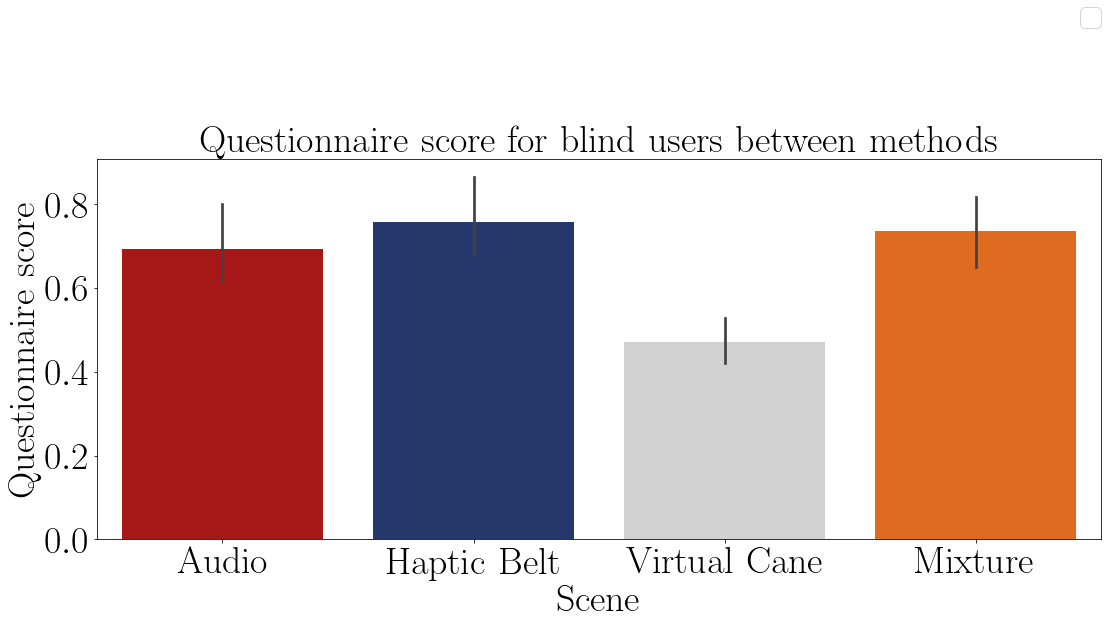
\includegraphics[width = 0.8\linewidth]{Resultados/Questionario/Figuras/png/barplot_questionnaire_scene_blind.png}
        %\resizebox{0.6\linewidth}{!}{
        %%% Creator: Matplotlib, PGF backend
%%
%% To include the figure in your LaTeX document, write
%%   \input{<filename>.pgf}
%%
%% Make sure the required packages are loaded in your preamble
%%   \usepackage{pgf}
%%
%% Figures using additional raster images can only be included by \input if
%% they are in the same directory as the main LaTeX file. For loading figures
%% from other directories you can use the `import` package
%%   \usepackage{import}
%%
%% and then include the figures with
%%   \import{<path to file>}{<filename>.pgf}
%%
%% Matplotlib used the following preamble
%%   \usepackage{fontspec}
%%
\begingroup%
\makeatletter%
\begin{pgfpicture}%
\pgfpathrectangle{\pgfpointorigin}{\pgfqpoint{15.185753in}{8.690562in}}%
\pgfusepath{use as bounding box, clip}%
\begin{pgfscope}%
\pgfsetbuttcap%
\pgfsetmiterjoin%
\pgfsetlinewidth{0.000000pt}%
\definecolor{currentstroke}{rgb}{1.000000,1.000000,1.000000}%
\pgfsetstrokecolor{currentstroke}%
\pgfsetstrokeopacity{0.000000}%
\pgfsetdash{}{0pt}%
\pgfpathmoveto{\pgfqpoint{0.000000in}{-0.000000in}}%
\pgfpathlineto{\pgfqpoint{15.185753in}{-0.000000in}}%
\pgfpathlineto{\pgfqpoint{15.185753in}{8.690562in}}%
\pgfpathlineto{\pgfqpoint{0.000000in}{8.690562in}}%
\pgfpathclose%
\pgfusepath{}%
\end{pgfscope}%
\begin{pgfscope}%
\pgfsetbuttcap%
\pgfsetmiterjoin%
\definecolor{currentfill}{rgb}{1.000000,1.000000,1.000000}%
\pgfsetfillcolor{currentfill}%
\pgfsetlinewidth{0.000000pt}%
\definecolor{currentstroke}{rgb}{0.000000,0.000000,0.000000}%
\pgfsetstrokecolor{currentstroke}%
\pgfsetstrokeopacity{0.000000}%
\pgfsetdash{}{0pt}%
\pgfpathmoveto{\pgfqpoint{1.135753in}{1.191562in}}%
\pgfpathlineto{\pgfqpoint{15.085753in}{1.191562in}}%
\pgfpathlineto{\pgfqpoint{15.085753in}{6.476562in}}%
\pgfpathlineto{\pgfqpoint{1.135753in}{6.476562in}}%
\pgfpathclose%
\pgfusepath{fill}%
\end{pgfscope}%
\begin{pgfscope}%
\pgfpathrectangle{\pgfqpoint{1.135753in}{1.191562in}}{\pgfqpoint{13.950000in}{5.285000in}}%
\pgfusepath{clip}%
\pgfsetbuttcap%
\pgfsetmiterjoin%
\definecolor{currentfill}{rgb}{0.651961,0.093137,0.093137}%
\pgfsetfillcolor{currentfill}%
\pgfsetlinewidth{0.000000pt}%
\definecolor{currentstroke}{rgb}{0.000000,0.000000,0.000000}%
\pgfsetstrokecolor{currentstroke}%
\pgfsetstrokeopacity{0.000000}%
\pgfsetdash{}{0pt}%
\pgfpathmoveto{\pgfqpoint{1.484503in}{1.191562in}}%
\pgfpathlineto{\pgfqpoint{4.274503in}{1.191562in}}%
\pgfpathlineto{\pgfqpoint{4.274503in}{5.230014in}}%
\pgfpathlineto{\pgfqpoint{1.484503in}{5.230014in}}%
\pgfpathclose%
\pgfusepath{fill}%
\end{pgfscope}%
\begin{pgfscope}%
\pgfpathrectangle{\pgfqpoint{1.135753in}{1.191562in}}{\pgfqpoint{13.950000in}{5.285000in}}%
\pgfusepath{clip}%
\pgfsetbuttcap%
\pgfsetmiterjoin%
\definecolor{currentfill}{rgb}{0.144608,0.218137,0.424020}%
\pgfsetfillcolor{currentfill}%
\pgfsetlinewidth{0.000000pt}%
\definecolor{currentstroke}{rgb}{0.000000,0.000000,0.000000}%
\pgfsetstrokecolor{currentstroke}%
\pgfsetstrokeopacity{0.000000}%
\pgfsetdash{}{0pt}%
\pgfpathmoveto{\pgfqpoint{4.972003in}{1.191562in}}%
\pgfpathlineto{\pgfqpoint{7.762003in}{1.191562in}}%
\pgfpathlineto{\pgfqpoint{7.762003in}{5.600928in}}%
\pgfpathlineto{\pgfqpoint{4.972003in}{5.600928in}}%
\pgfpathclose%
\pgfusepath{fill}%
\end{pgfscope}%
\begin{pgfscope}%
\pgfpathrectangle{\pgfqpoint{1.135753in}{1.191562in}}{\pgfqpoint{13.950000in}{5.285000in}}%
\pgfusepath{clip}%
\pgfsetbuttcap%
\pgfsetmiterjoin%
\definecolor{currentfill}{rgb}{0.823529,0.823529,0.823529}%
\pgfsetfillcolor{currentfill}%
\pgfsetlinewidth{0.000000pt}%
\definecolor{currentstroke}{rgb}{0.000000,0.000000,0.000000}%
\pgfsetstrokecolor{currentstroke}%
\pgfsetstrokeopacity{0.000000}%
\pgfsetdash{}{0pt}%
\pgfpathmoveto{\pgfqpoint{8.459503in}{1.191562in}}%
\pgfpathlineto{\pgfqpoint{11.249503in}{1.191562in}}%
\pgfpathlineto{\pgfqpoint{11.249503in}{3.937016in}}%
\pgfpathlineto{\pgfqpoint{8.459503in}{3.937016in}}%
\pgfpathclose%
\pgfusepath{fill}%
\end{pgfscope}%
\begin{pgfscope}%
\pgfpathrectangle{\pgfqpoint{1.135753in}{1.191562in}}{\pgfqpoint{13.950000in}{5.285000in}}%
\pgfusepath{clip}%
\pgfsetbuttcap%
\pgfsetmiterjoin%
\definecolor{currentfill}{rgb}{0.875000,0.419118,0.125000}%
\pgfsetfillcolor{currentfill}%
\pgfsetlinewidth{0.000000pt}%
\definecolor{currentstroke}{rgb}{0.000000,0.000000,0.000000}%
\pgfsetstrokecolor{currentstroke}%
\pgfsetstrokeopacity{0.000000}%
\pgfsetdash{}{0pt}%
\pgfpathmoveto{\pgfqpoint{11.947003in}{1.191562in}}%
\pgfpathlineto{\pgfqpoint{14.737003in}{1.191562in}}%
\pgfpathlineto{\pgfqpoint{14.737003in}{5.474877in}}%
\pgfpathlineto{\pgfqpoint{11.947003in}{5.474877in}}%
\pgfpathclose%
\pgfusepath{fill}%
\end{pgfscope}%
\begin{pgfscope}%
\pgfsetbuttcap%
\pgfsetroundjoin%
\definecolor{currentfill}{rgb}{0.000000,0.000000,0.000000}%
\pgfsetfillcolor{currentfill}%
\pgfsetlinewidth{0.803000pt}%
\definecolor{currentstroke}{rgb}{0.000000,0.000000,0.000000}%
\pgfsetstrokecolor{currentstroke}%
\pgfsetdash{}{0pt}%
\pgfsys@defobject{currentmarker}{\pgfqpoint{0.000000in}{-0.048611in}}{\pgfqpoint{0.000000in}{0.000000in}}{%
\pgfpathmoveto{\pgfqpoint{0.000000in}{0.000000in}}%
\pgfpathlineto{\pgfqpoint{0.000000in}{-0.048611in}}%
\pgfusepath{stroke,fill}%
}%
\begin{pgfscope}%
\pgfsys@transformshift{2.879503in}{1.191562in}%
\pgfsys@useobject{currentmarker}{}%
\end{pgfscope}%
\end{pgfscope}%
\begin{pgfscope}%
\definecolor{textcolor}{rgb}{0.000000,0.000000,0.000000}%
\pgfsetstrokecolor{textcolor}%
\pgfsetfillcolor{textcolor}%
\pgftext[x=2.879503in,y=1.094339in,,top]{\color{textcolor}\rmfamily\fontsize{38.016000}{45.619200}\selectfont Audio}%
\end{pgfscope}%
\begin{pgfscope}%
\pgfsetbuttcap%
\pgfsetroundjoin%
\definecolor{currentfill}{rgb}{0.000000,0.000000,0.000000}%
\pgfsetfillcolor{currentfill}%
\pgfsetlinewidth{0.803000pt}%
\definecolor{currentstroke}{rgb}{0.000000,0.000000,0.000000}%
\pgfsetstrokecolor{currentstroke}%
\pgfsetdash{}{0pt}%
\pgfsys@defobject{currentmarker}{\pgfqpoint{0.000000in}{-0.048611in}}{\pgfqpoint{0.000000in}{0.000000in}}{%
\pgfpathmoveto{\pgfqpoint{0.000000in}{0.000000in}}%
\pgfpathlineto{\pgfqpoint{0.000000in}{-0.048611in}}%
\pgfusepath{stroke,fill}%
}%
\begin{pgfscope}%
\pgfsys@transformshift{6.367003in}{1.191562in}%
\pgfsys@useobject{currentmarker}{}%
\end{pgfscope}%
\end{pgfscope}%
\begin{pgfscope}%
\definecolor{textcolor}{rgb}{0.000000,0.000000,0.000000}%
\pgfsetstrokecolor{textcolor}%
\pgfsetfillcolor{textcolor}%
\pgftext[x=6.367003in,y=1.094339in,,top]{\color{textcolor}\rmfamily\fontsize{38.016000}{45.619200}\selectfont Haptic Belt}%
\end{pgfscope}%
\begin{pgfscope}%
\pgfsetbuttcap%
\pgfsetroundjoin%
\definecolor{currentfill}{rgb}{0.000000,0.000000,0.000000}%
\pgfsetfillcolor{currentfill}%
\pgfsetlinewidth{0.803000pt}%
\definecolor{currentstroke}{rgb}{0.000000,0.000000,0.000000}%
\pgfsetstrokecolor{currentstroke}%
\pgfsetdash{}{0pt}%
\pgfsys@defobject{currentmarker}{\pgfqpoint{0.000000in}{-0.048611in}}{\pgfqpoint{0.000000in}{0.000000in}}{%
\pgfpathmoveto{\pgfqpoint{0.000000in}{0.000000in}}%
\pgfpathlineto{\pgfqpoint{0.000000in}{-0.048611in}}%
\pgfusepath{stroke,fill}%
}%
\begin{pgfscope}%
\pgfsys@transformshift{9.854503in}{1.191562in}%
\pgfsys@useobject{currentmarker}{}%
\end{pgfscope}%
\end{pgfscope}%
\begin{pgfscope}%
\definecolor{textcolor}{rgb}{0.000000,0.000000,0.000000}%
\pgfsetstrokecolor{textcolor}%
\pgfsetfillcolor{textcolor}%
\pgftext[x=9.854503in,y=1.094339in,,top]{\color{textcolor}\rmfamily\fontsize{38.016000}{45.619200}\selectfont Virtual Cane}%
\end{pgfscope}%
\begin{pgfscope}%
\pgfsetbuttcap%
\pgfsetroundjoin%
\definecolor{currentfill}{rgb}{0.000000,0.000000,0.000000}%
\pgfsetfillcolor{currentfill}%
\pgfsetlinewidth{0.803000pt}%
\definecolor{currentstroke}{rgb}{0.000000,0.000000,0.000000}%
\pgfsetstrokecolor{currentstroke}%
\pgfsetdash{}{0pt}%
\pgfsys@defobject{currentmarker}{\pgfqpoint{0.000000in}{-0.048611in}}{\pgfqpoint{0.000000in}{0.000000in}}{%
\pgfpathmoveto{\pgfqpoint{0.000000in}{0.000000in}}%
\pgfpathlineto{\pgfqpoint{0.000000in}{-0.048611in}}%
\pgfusepath{stroke,fill}%
}%
\begin{pgfscope}%
\pgfsys@transformshift{13.342003in}{1.191562in}%
\pgfsys@useobject{currentmarker}{}%
\end{pgfscope}%
\end{pgfscope}%
\begin{pgfscope}%
\definecolor{textcolor}{rgb}{0.000000,0.000000,0.000000}%
\pgfsetstrokecolor{textcolor}%
\pgfsetfillcolor{textcolor}%
\pgftext[x=13.342003in,y=1.094339in,,top]{\color{textcolor}\rmfamily\fontsize{38.016000}{45.619200}\selectfont Mixture}%
\end{pgfscope}%
\begin{pgfscope}%
\definecolor{textcolor}{rgb}{0.000000,0.000000,0.000000}%
\pgfsetstrokecolor{textcolor}%
\pgfsetfillcolor{textcolor}%
\pgftext[x=8.110753in,y=0.569392in,,top]{\color{textcolor}\rmfamily\fontsize{38.016000}{45.619200}\selectfont Scene}%
\end{pgfscope}%
\begin{pgfscope}%
\pgfsetbuttcap%
\pgfsetroundjoin%
\definecolor{currentfill}{rgb}{0.000000,0.000000,0.000000}%
\pgfsetfillcolor{currentfill}%
\pgfsetlinewidth{0.803000pt}%
\definecolor{currentstroke}{rgb}{0.000000,0.000000,0.000000}%
\pgfsetstrokecolor{currentstroke}%
\pgfsetdash{}{0pt}%
\pgfsys@defobject{currentmarker}{\pgfqpoint{-0.048611in}{0.000000in}}{\pgfqpoint{-0.000000in}{0.000000in}}{%
\pgfpathmoveto{\pgfqpoint{-0.000000in}{0.000000in}}%
\pgfpathlineto{\pgfqpoint{-0.048611in}{0.000000in}}%
\pgfusepath{stroke,fill}%
}%
\begin{pgfscope}%
\pgfsys@transformshift{1.135753in}{1.191562in}%
\pgfsys@useobject{currentmarker}{}%
\end{pgfscope}%
\end{pgfscope}%
\begin{pgfscope}%
\definecolor{textcolor}{rgb}{0.000000,0.000000,0.000000}%
\pgfsetstrokecolor{textcolor}%
\pgfsetfillcolor{textcolor}%
\pgftext[x=0.627588in, y=1.008346in, left, base]{\color{textcolor}\rmfamily\fontsize{38.016000}{45.619200}\selectfont \(\displaystyle {0.0}\)}%
\end{pgfscope}%
\begin{pgfscope}%
\pgfsetbuttcap%
\pgfsetroundjoin%
\definecolor{currentfill}{rgb}{0.000000,0.000000,0.000000}%
\pgfsetfillcolor{currentfill}%
\pgfsetlinewidth{0.803000pt}%
\definecolor{currentstroke}{rgb}{0.000000,0.000000,0.000000}%
\pgfsetstrokecolor{currentstroke}%
\pgfsetdash{}{0pt}%
\pgfsys@defobject{currentmarker}{\pgfqpoint{-0.048611in}{0.000000in}}{\pgfqpoint{-0.000000in}{0.000000in}}{%
\pgfpathmoveto{\pgfqpoint{-0.000000in}{0.000000in}}%
\pgfpathlineto{\pgfqpoint{-0.048611in}{0.000000in}}%
\pgfusepath{stroke,fill}%
}%
\begin{pgfscope}%
\pgfsys@transformshift{1.135753in}{2.356300in}%
\pgfsys@useobject{currentmarker}{}%
\end{pgfscope}%
\end{pgfscope}%
\begin{pgfscope}%
\definecolor{textcolor}{rgb}{0.000000,0.000000,0.000000}%
\pgfsetstrokecolor{textcolor}%
\pgfsetfillcolor{textcolor}%
\pgftext[x=0.627588in, y=2.173084in, left, base]{\color{textcolor}\rmfamily\fontsize{38.016000}{45.619200}\selectfont \(\displaystyle {0.2}\)}%
\end{pgfscope}%
\begin{pgfscope}%
\pgfsetbuttcap%
\pgfsetroundjoin%
\definecolor{currentfill}{rgb}{0.000000,0.000000,0.000000}%
\pgfsetfillcolor{currentfill}%
\pgfsetlinewidth{0.803000pt}%
\definecolor{currentstroke}{rgb}{0.000000,0.000000,0.000000}%
\pgfsetstrokecolor{currentstroke}%
\pgfsetdash{}{0pt}%
\pgfsys@defobject{currentmarker}{\pgfqpoint{-0.048611in}{0.000000in}}{\pgfqpoint{-0.000000in}{0.000000in}}{%
\pgfpathmoveto{\pgfqpoint{-0.000000in}{0.000000in}}%
\pgfpathlineto{\pgfqpoint{-0.048611in}{0.000000in}}%
\pgfusepath{stroke,fill}%
}%
\begin{pgfscope}%
\pgfsys@transformshift{1.135753in}{3.521038in}%
\pgfsys@useobject{currentmarker}{}%
\end{pgfscope}%
\end{pgfscope}%
\begin{pgfscope}%
\definecolor{textcolor}{rgb}{0.000000,0.000000,0.000000}%
\pgfsetstrokecolor{textcolor}%
\pgfsetfillcolor{textcolor}%
\pgftext[x=0.627588in, y=3.337822in, left, base]{\color{textcolor}\rmfamily\fontsize{38.016000}{45.619200}\selectfont \(\displaystyle {0.4}\)}%
\end{pgfscope}%
\begin{pgfscope}%
\pgfsetbuttcap%
\pgfsetroundjoin%
\definecolor{currentfill}{rgb}{0.000000,0.000000,0.000000}%
\pgfsetfillcolor{currentfill}%
\pgfsetlinewidth{0.803000pt}%
\definecolor{currentstroke}{rgb}{0.000000,0.000000,0.000000}%
\pgfsetstrokecolor{currentstroke}%
\pgfsetdash{}{0pt}%
\pgfsys@defobject{currentmarker}{\pgfqpoint{-0.048611in}{0.000000in}}{\pgfqpoint{-0.000000in}{0.000000in}}{%
\pgfpathmoveto{\pgfqpoint{-0.000000in}{0.000000in}}%
\pgfpathlineto{\pgfqpoint{-0.048611in}{0.000000in}}%
\pgfusepath{stroke,fill}%
}%
\begin{pgfscope}%
\pgfsys@transformshift{1.135753in}{4.685777in}%
\pgfsys@useobject{currentmarker}{}%
\end{pgfscope}%
\end{pgfscope}%
\begin{pgfscope}%
\definecolor{textcolor}{rgb}{0.000000,0.000000,0.000000}%
\pgfsetstrokecolor{textcolor}%
\pgfsetfillcolor{textcolor}%
\pgftext[x=0.627588in, y=4.502560in, left, base]{\color{textcolor}\rmfamily\fontsize{38.016000}{45.619200}\selectfont \(\displaystyle {0.6}\)}%
\end{pgfscope}%
\begin{pgfscope}%
\pgfsetbuttcap%
\pgfsetroundjoin%
\definecolor{currentfill}{rgb}{0.000000,0.000000,0.000000}%
\pgfsetfillcolor{currentfill}%
\pgfsetlinewidth{0.803000pt}%
\definecolor{currentstroke}{rgb}{0.000000,0.000000,0.000000}%
\pgfsetstrokecolor{currentstroke}%
\pgfsetdash{}{0pt}%
\pgfsys@defobject{currentmarker}{\pgfqpoint{-0.048611in}{0.000000in}}{\pgfqpoint{-0.000000in}{0.000000in}}{%
\pgfpathmoveto{\pgfqpoint{-0.000000in}{0.000000in}}%
\pgfpathlineto{\pgfqpoint{-0.048611in}{0.000000in}}%
\pgfusepath{stroke,fill}%
}%
\begin{pgfscope}%
\pgfsys@transformshift{1.135753in}{5.850515in}%
\pgfsys@useobject{currentmarker}{}%
\end{pgfscope}%
\end{pgfscope}%
\begin{pgfscope}%
\definecolor{textcolor}{rgb}{0.000000,0.000000,0.000000}%
\pgfsetstrokecolor{textcolor}%
\pgfsetfillcolor{textcolor}%
\pgftext[x=0.627588in, y=5.667299in, left, base]{\color{textcolor}\rmfamily\fontsize{38.016000}{45.619200}\selectfont \(\displaystyle {0.8}\)}%
\end{pgfscope}%
\begin{pgfscope}%
\definecolor{textcolor}{rgb}{0.000000,0.000000,0.000000}%
\pgfsetstrokecolor{textcolor}%
\pgfsetfillcolor{textcolor}%
\pgftext[x=0.572032in,y=3.834062in,,bottom,rotate=90.000000]{\color{textcolor}\rmfamily\fontsize{38.016000}{45.619200}\selectfont Questionnaire score}%
\end{pgfscope}%
\begin{pgfscope}%
\pgfpathrectangle{\pgfqpoint{1.135753in}{1.191562in}}{\pgfqpoint{13.950000in}{5.285000in}}%
\pgfusepath{clip}%
\pgfsetrectcap%
\pgfsetroundjoin%
\pgfsetlinewidth{2.710125pt}%
\definecolor{currentstroke}{rgb}{0.260000,0.260000,0.260000}%
\pgfsetstrokecolor{currentstroke}%
\pgfsetdash{}{0pt}%
\pgfpathmoveto{\pgfqpoint{2.879503in}{4.710042in}}%
\pgfpathlineto{\pgfqpoint{2.879503in}{5.940643in}}%
\pgfusepath{stroke}%
\end{pgfscope}%
\begin{pgfscope}%
\pgfpathrectangle{\pgfqpoint{1.135753in}{1.191562in}}{\pgfqpoint{13.950000in}{5.285000in}}%
\pgfusepath{clip}%
\pgfsetrectcap%
\pgfsetroundjoin%
\pgfsetlinewidth{2.710125pt}%
\definecolor{currentstroke}{rgb}{0.260000,0.260000,0.260000}%
\pgfsetstrokecolor{currentstroke}%
\pgfsetdash{}{0pt}%
\pgfpathmoveto{\pgfqpoint{6.367003in}{5.143352in}}%
\pgfpathlineto{\pgfqpoint{6.367003in}{6.224895in}}%
\pgfusepath{stroke}%
\end{pgfscope}%
\begin{pgfscope}%
\pgfpathrectangle{\pgfqpoint{1.135753in}{1.191562in}}{\pgfqpoint{13.950000in}{5.285000in}}%
\pgfusepath{clip}%
\pgfsetrectcap%
\pgfsetroundjoin%
\pgfsetlinewidth{2.710125pt}%
\definecolor{currentstroke}{rgb}{0.260000,0.260000,0.260000}%
\pgfsetstrokecolor{currentstroke}%
\pgfsetdash{}{0pt}%
\pgfpathmoveto{\pgfqpoint{9.854503in}{3.645832in}}%
\pgfpathlineto{\pgfqpoint{9.854503in}{4.269799in}}%
\pgfusepath{stroke}%
\end{pgfscope}%
\begin{pgfscope}%
\pgfpathrectangle{\pgfqpoint{1.135753in}{1.191562in}}{\pgfqpoint{13.950000in}{5.285000in}}%
\pgfusepath{clip}%
\pgfsetrectcap%
\pgfsetroundjoin%
\pgfsetlinewidth{2.710125pt}%
\definecolor{currentstroke}{rgb}{0.260000,0.260000,0.260000}%
\pgfsetstrokecolor{currentstroke}%
\pgfsetdash{}{0pt}%
\pgfpathmoveto{\pgfqpoint{13.342003in}{4.970028in}}%
\pgfpathlineto{\pgfqpoint{13.342003in}{6.007934in}}%
\pgfusepath{stroke}%
\end{pgfscope}%
\begin{pgfscope}%
\pgfsetrectcap%
\pgfsetmiterjoin%
\pgfsetlinewidth{0.803000pt}%
\definecolor{currentstroke}{rgb}{0.000000,0.000000,0.000000}%
\pgfsetstrokecolor{currentstroke}%
\pgfsetdash{}{0pt}%
\pgfpathmoveto{\pgfqpoint{1.135753in}{1.191562in}}%
\pgfpathlineto{\pgfqpoint{1.135753in}{6.476562in}}%
\pgfusepath{stroke}%
\end{pgfscope}%
\begin{pgfscope}%
\pgfsetrectcap%
\pgfsetmiterjoin%
\pgfsetlinewidth{0.803000pt}%
\definecolor{currentstroke}{rgb}{0.000000,0.000000,0.000000}%
\pgfsetstrokecolor{currentstroke}%
\pgfsetdash{}{0pt}%
\pgfpathmoveto{\pgfqpoint{15.085753in}{1.191562in}}%
\pgfpathlineto{\pgfqpoint{15.085753in}{6.476562in}}%
\pgfusepath{stroke}%
\end{pgfscope}%
\begin{pgfscope}%
\pgfsetrectcap%
\pgfsetmiterjoin%
\pgfsetlinewidth{0.803000pt}%
\definecolor{currentstroke}{rgb}{0.000000,0.000000,0.000000}%
\pgfsetstrokecolor{currentstroke}%
\pgfsetdash{}{0pt}%
\pgfpathmoveto{\pgfqpoint{1.135753in}{1.191562in}}%
\pgfpathlineto{\pgfqpoint{15.085753in}{1.191562in}}%
\pgfusepath{stroke}%
\end{pgfscope}%
\begin{pgfscope}%
\pgfsetrectcap%
\pgfsetmiterjoin%
\pgfsetlinewidth{0.803000pt}%
\definecolor{currentstroke}{rgb}{0.000000,0.000000,0.000000}%
\pgfsetstrokecolor{currentstroke}%
\pgfsetdash{}{0pt}%
\pgfpathmoveto{\pgfqpoint{1.135753in}{6.476562in}}%
\pgfpathlineto{\pgfqpoint{15.085753in}{6.476562in}}%
\pgfusepath{stroke}%
\end{pgfscope}%
\begin{pgfscope}%
\definecolor{textcolor}{rgb}{0.000000,0.000000,0.000000}%
\pgfsetstrokecolor{textcolor}%
\pgfsetfillcolor{textcolor}%
\pgftext[x=8.110753in,y=6.579521in,,base]{\color{textcolor}\rmfamily\fontsize{38.016000}{45.619200}\selectfont Questionnaire score for blind users between methods}%
\end{pgfscope}%
\begin{pgfscope}%
\pgfsetbuttcap%
\pgfsetmiterjoin%
\definecolor{currentfill}{rgb}{1.000000,1.000000,1.000000}%
\pgfsetfillcolor{currentfill}%
\pgfsetfillopacity{0.800000}%
\pgfsetlinewidth{1.003750pt}%
\definecolor{currentstroke}{rgb}{0.800000,0.800000,0.800000}%
\pgfsetstrokecolor{currentstroke}%
\pgfsetstrokeopacity{0.800000}%
\pgfsetdash{}{0pt}%
\pgfpathmoveto{\pgfqpoint{14.865753in}{8.297228in}}%
\pgfpathlineto{\pgfqpoint{15.012419in}{8.297228in}}%
\pgfpathquadraticcurveto{\pgfqpoint{15.085753in}{8.297228in}}{\pgfqpoint{15.085753in}{8.370562in}}%
\pgfpathlineto{\pgfqpoint{15.085753in}{8.517228in}}%
\pgfpathquadraticcurveto{\pgfqpoint{15.085753in}{8.590562in}}{\pgfqpoint{15.012419in}{8.590562in}}%
\pgfpathlineto{\pgfqpoint{14.865753in}{8.590562in}}%
\pgfpathquadraticcurveto{\pgfqpoint{14.792419in}{8.590562in}}{\pgfqpoint{14.792419in}{8.517228in}}%
\pgfpathlineto{\pgfqpoint{14.792419in}{8.370562in}}%
\pgfpathquadraticcurveto{\pgfqpoint{14.792419in}{8.297228in}}{\pgfqpoint{14.865753in}{8.297228in}}%
\pgfpathclose%
\pgfusepath{stroke,fill}%
\end{pgfscope}%
\end{pgfpicture}%
\makeatother%
\endgroup%
    
        %}
        \caption{Bar plot of the average mental demand of the blind participants on each method.}
        \label{fig:barplot_questionnaire_scene_blind}
    \end{minipage}
    \begin{minipage}{\textwidth}
        \centering
        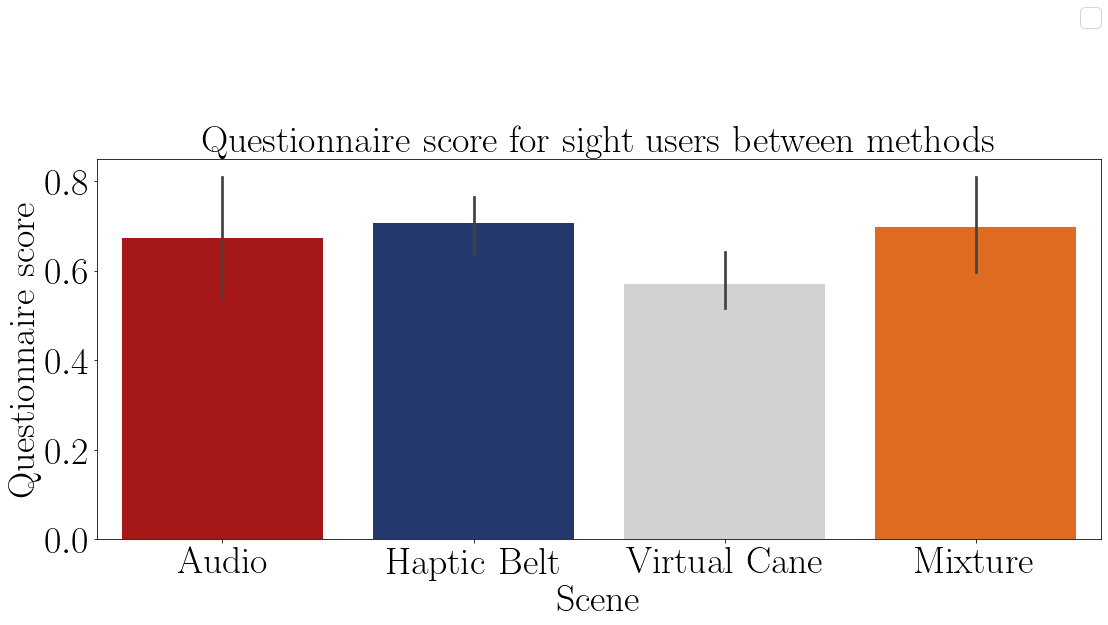
\includegraphics[width = 0.8\linewidth]{Resultados/Questionario/Figuras/png/barplot_questionnaire_scene_sight.png}
        %\resizebox{0.6\linewidth}{!}{
        %%% Creator: Matplotlib, PGF backend
%%
%% To include the figure in your LaTeX document, write
%%   \input{<filename>.pgf}
%%
%% Make sure the required packages are loaded in your preamble
%%   \usepackage{pgf}
%%
%% Figures using additional raster images can only be included by \input if
%% they are in the same directory as the main LaTeX file. For loading figures
%% from other directories you can use the `import` package
%%   \usepackage{import}
%%
%% and then include the figures with
%%   \import{<path to file>}{<filename>.pgf}
%%
%% Matplotlib used the following preamble
%%   \usepackage{fontspec}
%%
\begingroup%
\makeatletter%
\begin{pgfpicture}%
\pgfpathrectangle{\pgfpointorigin}{\pgfqpoint{15.185753in}{8.690562in}}%
\pgfusepath{use as bounding box, clip}%
\begin{pgfscope}%
\pgfsetbuttcap%
\pgfsetmiterjoin%
\pgfsetlinewidth{0.000000pt}%
\definecolor{currentstroke}{rgb}{1.000000,1.000000,1.000000}%
\pgfsetstrokecolor{currentstroke}%
\pgfsetstrokeopacity{0.000000}%
\pgfsetdash{}{0pt}%
\pgfpathmoveto{\pgfqpoint{0.000000in}{-0.000000in}}%
\pgfpathlineto{\pgfqpoint{15.185753in}{-0.000000in}}%
\pgfpathlineto{\pgfqpoint{15.185753in}{8.690562in}}%
\pgfpathlineto{\pgfqpoint{0.000000in}{8.690562in}}%
\pgfpathclose%
\pgfusepath{}%
\end{pgfscope}%
\begin{pgfscope}%
\pgfsetbuttcap%
\pgfsetmiterjoin%
\definecolor{currentfill}{rgb}{1.000000,1.000000,1.000000}%
\pgfsetfillcolor{currentfill}%
\pgfsetlinewidth{0.000000pt}%
\definecolor{currentstroke}{rgb}{0.000000,0.000000,0.000000}%
\pgfsetstrokecolor{currentstroke}%
\pgfsetstrokeopacity{0.000000}%
\pgfsetdash{}{0pt}%
\pgfpathmoveto{\pgfqpoint{1.135753in}{1.191562in}}%
\pgfpathlineto{\pgfqpoint{15.085753in}{1.191562in}}%
\pgfpathlineto{\pgfqpoint{15.085753in}{6.476562in}}%
\pgfpathlineto{\pgfqpoint{1.135753in}{6.476562in}}%
\pgfpathclose%
\pgfusepath{fill}%
\end{pgfscope}%
\begin{pgfscope}%
\pgfpathrectangle{\pgfqpoint{1.135753in}{1.191562in}}{\pgfqpoint{13.950000in}{5.285000in}}%
\pgfusepath{clip}%
\pgfsetbuttcap%
\pgfsetmiterjoin%
\definecolor{currentfill}{rgb}{0.651961,0.093137,0.093137}%
\pgfsetfillcolor{currentfill}%
\pgfsetlinewidth{0.000000pt}%
\definecolor{currentstroke}{rgb}{0.000000,0.000000,0.000000}%
\pgfsetstrokecolor{currentstroke}%
\pgfsetstrokeopacity{0.000000}%
\pgfsetdash{}{0pt}%
\pgfpathmoveto{\pgfqpoint{1.484503in}{1.191562in}}%
\pgfpathlineto{\pgfqpoint{4.274503in}{1.191562in}}%
\pgfpathlineto{\pgfqpoint{4.274503in}{5.710737in}}%
\pgfpathlineto{\pgfqpoint{1.484503in}{5.710737in}}%
\pgfpathclose%
\pgfusepath{fill}%
\end{pgfscope}%
\begin{pgfscope}%
\pgfpathrectangle{\pgfqpoint{1.135753in}{1.191562in}}{\pgfqpoint{13.950000in}{5.285000in}}%
\pgfusepath{clip}%
\pgfsetbuttcap%
\pgfsetmiterjoin%
\definecolor{currentfill}{rgb}{0.144608,0.218137,0.424020}%
\pgfsetfillcolor{currentfill}%
\pgfsetlinewidth{0.000000pt}%
\definecolor{currentstroke}{rgb}{0.000000,0.000000,0.000000}%
\pgfsetstrokecolor{currentstroke}%
\pgfsetstrokeopacity{0.000000}%
\pgfsetdash{}{0pt}%
\pgfpathmoveto{\pgfqpoint{4.972003in}{1.191562in}}%
\pgfpathlineto{\pgfqpoint{7.762003in}{1.191562in}}%
\pgfpathlineto{\pgfqpoint{7.762003in}{4.525468in}}%
\pgfpathlineto{\pgfqpoint{4.972003in}{4.525468in}}%
\pgfpathclose%
\pgfusepath{fill}%
\end{pgfscope}%
\begin{pgfscope}%
\pgfpathrectangle{\pgfqpoint{1.135753in}{1.191562in}}{\pgfqpoint{13.950000in}{5.285000in}}%
\pgfusepath{clip}%
\pgfsetbuttcap%
\pgfsetmiterjoin%
\definecolor{currentfill}{rgb}{0.823529,0.823529,0.823529}%
\pgfsetfillcolor{currentfill}%
\pgfsetlinewidth{0.000000pt}%
\definecolor{currentstroke}{rgb}{0.000000,0.000000,0.000000}%
\pgfsetstrokecolor{currentstroke}%
\pgfsetstrokeopacity{0.000000}%
\pgfsetdash{}{0pt}%
\pgfpathmoveto{\pgfqpoint{8.459503in}{1.191562in}}%
\pgfpathlineto{\pgfqpoint{11.249503in}{1.191562in}}%
\pgfpathlineto{\pgfqpoint{11.249503in}{5.196580in}}%
\pgfpathlineto{\pgfqpoint{8.459503in}{5.196580in}}%
\pgfpathclose%
\pgfusepath{fill}%
\end{pgfscope}%
\begin{pgfscope}%
\pgfpathrectangle{\pgfqpoint{1.135753in}{1.191562in}}{\pgfqpoint{13.950000in}{5.285000in}}%
\pgfusepath{clip}%
\pgfsetbuttcap%
\pgfsetmiterjoin%
\definecolor{currentfill}{rgb}{0.875000,0.419118,0.125000}%
\pgfsetfillcolor{currentfill}%
\pgfsetlinewidth{0.000000pt}%
\definecolor{currentstroke}{rgb}{0.000000,0.000000,0.000000}%
\pgfsetstrokecolor{currentstroke}%
\pgfsetstrokeopacity{0.000000}%
\pgfsetdash{}{0pt}%
\pgfpathmoveto{\pgfqpoint{11.947003in}{1.191562in}}%
\pgfpathlineto{\pgfqpoint{14.737003in}{1.191562in}}%
\pgfpathlineto{\pgfqpoint{14.737003in}{5.860634in}}%
\pgfpathlineto{\pgfqpoint{11.947003in}{5.860634in}}%
\pgfpathclose%
\pgfusepath{fill}%
\end{pgfscope}%
\begin{pgfscope}%
\pgfsetbuttcap%
\pgfsetroundjoin%
\definecolor{currentfill}{rgb}{0.000000,0.000000,0.000000}%
\pgfsetfillcolor{currentfill}%
\pgfsetlinewidth{0.803000pt}%
\definecolor{currentstroke}{rgb}{0.000000,0.000000,0.000000}%
\pgfsetstrokecolor{currentstroke}%
\pgfsetdash{}{0pt}%
\pgfsys@defobject{currentmarker}{\pgfqpoint{0.000000in}{-0.048611in}}{\pgfqpoint{0.000000in}{0.000000in}}{%
\pgfpathmoveto{\pgfqpoint{0.000000in}{0.000000in}}%
\pgfpathlineto{\pgfqpoint{0.000000in}{-0.048611in}}%
\pgfusepath{stroke,fill}%
}%
\begin{pgfscope}%
\pgfsys@transformshift{2.879503in}{1.191562in}%
\pgfsys@useobject{currentmarker}{}%
\end{pgfscope}%
\end{pgfscope}%
\begin{pgfscope}%
\definecolor{textcolor}{rgb}{0.000000,0.000000,0.000000}%
\pgfsetstrokecolor{textcolor}%
\pgfsetfillcolor{textcolor}%
\pgftext[x=2.879503in,y=1.094339in,,top]{\color{textcolor}\rmfamily\fontsize{38.016000}{45.619200}\selectfont Audio}%
\end{pgfscope}%
\begin{pgfscope}%
\pgfsetbuttcap%
\pgfsetroundjoin%
\definecolor{currentfill}{rgb}{0.000000,0.000000,0.000000}%
\pgfsetfillcolor{currentfill}%
\pgfsetlinewidth{0.803000pt}%
\definecolor{currentstroke}{rgb}{0.000000,0.000000,0.000000}%
\pgfsetstrokecolor{currentstroke}%
\pgfsetdash{}{0pt}%
\pgfsys@defobject{currentmarker}{\pgfqpoint{0.000000in}{-0.048611in}}{\pgfqpoint{0.000000in}{0.000000in}}{%
\pgfpathmoveto{\pgfqpoint{0.000000in}{0.000000in}}%
\pgfpathlineto{\pgfqpoint{0.000000in}{-0.048611in}}%
\pgfusepath{stroke,fill}%
}%
\begin{pgfscope}%
\pgfsys@transformshift{6.367003in}{1.191562in}%
\pgfsys@useobject{currentmarker}{}%
\end{pgfscope}%
\end{pgfscope}%
\begin{pgfscope}%
\definecolor{textcolor}{rgb}{0.000000,0.000000,0.000000}%
\pgfsetstrokecolor{textcolor}%
\pgfsetfillcolor{textcolor}%
\pgftext[x=6.367003in,y=1.094339in,,top]{\color{textcolor}\rmfamily\fontsize{38.016000}{45.619200}\selectfont Haptic Belt}%
\end{pgfscope}%
\begin{pgfscope}%
\pgfsetbuttcap%
\pgfsetroundjoin%
\definecolor{currentfill}{rgb}{0.000000,0.000000,0.000000}%
\pgfsetfillcolor{currentfill}%
\pgfsetlinewidth{0.803000pt}%
\definecolor{currentstroke}{rgb}{0.000000,0.000000,0.000000}%
\pgfsetstrokecolor{currentstroke}%
\pgfsetdash{}{0pt}%
\pgfsys@defobject{currentmarker}{\pgfqpoint{0.000000in}{-0.048611in}}{\pgfqpoint{0.000000in}{0.000000in}}{%
\pgfpathmoveto{\pgfqpoint{0.000000in}{0.000000in}}%
\pgfpathlineto{\pgfqpoint{0.000000in}{-0.048611in}}%
\pgfusepath{stroke,fill}%
}%
\begin{pgfscope}%
\pgfsys@transformshift{9.854503in}{1.191562in}%
\pgfsys@useobject{currentmarker}{}%
\end{pgfscope}%
\end{pgfscope}%
\begin{pgfscope}%
\definecolor{textcolor}{rgb}{0.000000,0.000000,0.000000}%
\pgfsetstrokecolor{textcolor}%
\pgfsetfillcolor{textcolor}%
\pgftext[x=9.854503in,y=1.094339in,,top]{\color{textcolor}\rmfamily\fontsize{38.016000}{45.619200}\selectfont Virtual Cane}%
\end{pgfscope}%
\begin{pgfscope}%
\pgfsetbuttcap%
\pgfsetroundjoin%
\definecolor{currentfill}{rgb}{0.000000,0.000000,0.000000}%
\pgfsetfillcolor{currentfill}%
\pgfsetlinewidth{0.803000pt}%
\definecolor{currentstroke}{rgb}{0.000000,0.000000,0.000000}%
\pgfsetstrokecolor{currentstroke}%
\pgfsetdash{}{0pt}%
\pgfsys@defobject{currentmarker}{\pgfqpoint{0.000000in}{-0.048611in}}{\pgfqpoint{0.000000in}{0.000000in}}{%
\pgfpathmoveto{\pgfqpoint{0.000000in}{0.000000in}}%
\pgfpathlineto{\pgfqpoint{0.000000in}{-0.048611in}}%
\pgfusepath{stroke,fill}%
}%
\begin{pgfscope}%
\pgfsys@transformshift{13.342003in}{1.191562in}%
\pgfsys@useobject{currentmarker}{}%
\end{pgfscope}%
\end{pgfscope}%
\begin{pgfscope}%
\definecolor{textcolor}{rgb}{0.000000,0.000000,0.000000}%
\pgfsetstrokecolor{textcolor}%
\pgfsetfillcolor{textcolor}%
\pgftext[x=13.342003in,y=1.094339in,,top]{\color{textcolor}\rmfamily\fontsize{38.016000}{45.619200}\selectfont Mixture}%
\end{pgfscope}%
\begin{pgfscope}%
\definecolor{textcolor}{rgb}{0.000000,0.000000,0.000000}%
\pgfsetstrokecolor{textcolor}%
\pgfsetfillcolor{textcolor}%
\pgftext[x=8.110753in,y=0.569392in,,top]{\color{textcolor}\rmfamily\fontsize{38.016000}{45.619200}\selectfont Scene}%
\end{pgfscope}%
\begin{pgfscope}%
\pgfsetbuttcap%
\pgfsetroundjoin%
\definecolor{currentfill}{rgb}{0.000000,0.000000,0.000000}%
\pgfsetfillcolor{currentfill}%
\pgfsetlinewidth{0.803000pt}%
\definecolor{currentstroke}{rgb}{0.000000,0.000000,0.000000}%
\pgfsetstrokecolor{currentstroke}%
\pgfsetdash{}{0pt}%
\pgfsys@defobject{currentmarker}{\pgfqpoint{-0.048611in}{0.000000in}}{\pgfqpoint{-0.000000in}{0.000000in}}{%
\pgfpathmoveto{\pgfqpoint{-0.000000in}{0.000000in}}%
\pgfpathlineto{\pgfqpoint{-0.048611in}{0.000000in}}%
\pgfusepath{stroke,fill}%
}%
\begin{pgfscope}%
\pgfsys@transformshift{1.135753in}{1.191562in}%
\pgfsys@useobject{currentmarker}{}%
\end{pgfscope}%
\end{pgfscope}%
\begin{pgfscope}%
\definecolor{textcolor}{rgb}{0.000000,0.000000,0.000000}%
\pgfsetstrokecolor{textcolor}%
\pgfsetfillcolor{textcolor}%
\pgftext[x=0.627588in, y=1.008346in, left, base]{\color{textcolor}\rmfamily\fontsize{38.016000}{45.619200}\selectfont \(\displaystyle {0.0}\)}%
\end{pgfscope}%
\begin{pgfscope}%
\pgfsetbuttcap%
\pgfsetroundjoin%
\definecolor{currentfill}{rgb}{0.000000,0.000000,0.000000}%
\pgfsetfillcolor{currentfill}%
\pgfsetlinewidth{0.803000pt}%
\definecolor{currentstroke}{rgb}{0.000000,0.000000,0.000000}%
\pgfsetstrokecolor{currentstroke}%
\pgfsetdash{}{0pt}%
\pgfsys@defobject{currentmarker}{\pgfqpoint{-0.048611in}{0.000000in}}{\pgfqpoint{-0.000000in}{0.000000in}}{%
\pgfpathmoveto{\pgfqpoint{-0.000000in}{0.000000in}}%
\pgfpathlineto{\pgfqpoint{-0.048611in}{0.000000in}}%
\pgfusepath{stroke,fill}%
}%
\begin{pgfscope}%
\pgfsys@transformshift{1.135753in}{2.403891in}%
\pgfsys@useobject{currentmarker}{}%
\end{pgfscope}%
\end{pgfscope}%
\begin{pgfscope}%
\definecolor{textcolor}{rgb}{0.000000,0.000000,0.000000}%
\pgfsetstrokecolor{textcolor}%
\pgfsetfillcolor{textcolor}%
\pgftext[x=0.627588in, y=2.220675in, left, base]{\color{textcolor}\rmfamily\fontsize{38.016000}{45.619200}\selectfont \(\displaystyle {0.2}\)}%
\end{pgfscope}%
\begin{pgfscope}%
\pgfsetbuttcap%
\pgfsetroundjoin%
\definecolor{currentfill}{rgb}{0.000000,0.000000,0.000000}%
\pgfsetfillcolor{currentfill}%
\pgfsetlinewidth{0.803000pt}%
\definecolor{currentstroke}{rgb}{0.000000,0.000000,0.000000}%
\pgfsetstrokecolor{currentstroke}%
\pgfsetdash{}{0pt}%
\pgfsys@defobject{currentmarker}{\pgfqpoint{-0.048611in}{0.000000in}}{\pgfqpoint{-0.000000in}{0.000000in}}{%
\pgfpathmoveto{\pgfqpoint{-0.000000in}{0.000000in}}%
\pgfpathlineto{\pgfqpoint{-0.048611in}{0.000000in}}%
\pgfusepath{stroke,fill}%
}%
\begin{pgfscope}%
\pgfsys@transformshift{1.135753in}{3.616221in}%
\pgfsys@useobject{currentmarker}{}%
\end{pgfscope}%
\end{pgfscope}%
\begin{pgfscope}%
\definecolor{textcolor}{rgb}{0.000000,0.000000,0.000000}%
\pgfsetstrokecolor{textcolor}%
\pgfsetfillcolor{textcolor}%
\pgftext[x=0.627588in, y=3.433005in, left, base]{\color{textcolor}\rmfamily\fontsize{38.016000}{45.619200}\selectfont \(\displaystyle {0.4}\)}%
\end{pgfscope}%
\begin{pgfscope}%
\pgfsetbuttcap%
\pgfsetroundjoin%
\definecolor{currentfill}{rgb}{0.000000,0.000000,0.000000}%
\pgfsetfillcolor{currentfill}%
\pgfsetlinewidth{0.803000pt}%
\definecolor{currentstroke}{rgb}{0.000000,0.000000,0.000000}%
\pgfsetstrokecolor{currentstroke}%
\pgfsetdash{}{0pt}%
\pgfsys@defobject{currentmarker}{\pgfqpoint{-0.048611in}{0.000000in}}{\pgfqpoint{-0.000000in}{0.000000in}}{%
\pgfpathmoveto{\pgfqpoint{-0.000000in}{0.000000in}}%
\pgfpathlineto{\pgfqpoint{-0.048611in}{0.000000in}}%
\pgfusepath{stroke,fill}%
}%
\begin{pgfscope}%
\pgfsys@transformshift{1.135753in}{4.828551in}%
\pgfsys@useobject{currentmarker}{}%
\end{pgfscope}%
\end{pgfscope}%
\begin{pgfscope}%
\definecolor{textcolor}{rgb}{0.000000,0.000000,0.000000}%
\pgfsetstrokecolor{textcolor}%
\pgfsetfillcolor{textcolor}%
\pgftext[x=0.627588in, y=4.645335in, left, base]{\color{textcolor}\rmfamily\fontsize{38.016000}{45.619200}\selectfont \(\displaystyle {0.6}\)}%
\end{pgfscope}%
\begin{pgfscope}%
\pgfsetbuttcap%
\pgfsetroundjoin%
\definecolor{currentfill}{rgb}{0.000000,0.000000,0.000000}%
\pgfsetfillcolor{currentfill}%
\pgfsetlinewidth{0.803000pt}%
\definecolor{currentstroke}{rgb}{0.000000,0.000000,0.000000}%
\pgfsetstrokecolor{currentstroke}%
\pgfsetdash{}{0pt}%
\pgfsys@defobject{currentmarker}{\pgfqpoint{-0.048611in}{0.000000in}}{\pgfqpoint{-0.000000in}{0.000000in}}{%
\pgfpathmoveto{\pgfqpoint{-0.000000in}{0.000000in}}%
\pgfpathlineto{\pgfqpoint{-0.048611in}{0.000000in}}%
\pgfusepath{stroke,fill}%
}%
\begin{pgfscope}%
\pgfsys@transformshift{1.135753in}{6.040881in}%
\pgfsys@useobject{currentmarker}{}%
\end{pgfscope}%
\end{pgfscope}%
\begin{pgfscope}%
\definecolor{textcolor}{rgb}{0.000000,0.000000,0.000000}%
\pgfsetstrokecolor{textcolor}%
\pgfsetfillcolor{textcolor}%
\pgftext[x=0.627588in, y=5.857665in, left, base]{\color{textcolor}\rmfamily\fontsize{38.016000}{45.619200}\selectfont \(\displaystyle {0.8}\)}%
\end{pgfscope}%
\begin{pgfscope}%
\definecolor{textcolor}{rgb}{0.000000,0.000000,0.000000}%
\pgfsetstrokecolor{textcolor}%
\pgfsetfillcolor{textcolor}%
\pgftext[x=0.572032in,y=3.834062in,,bottom,rotate=90.000000]{\color{textcolor}\rmfamily\fontsize{38.016000}{45.619200}\selectfont Questionnaire score}%
\end{pgfscope}%
\begin{pgfscope}%
\pgfpathrectangle{\pgfqpoint{1.135753in}{1.191562in}}{\pgfqpoint{13.950000in}{5.285000in}}%
\pgfusepath{clip}%
\pgfsetrectcap%
\pgfsetroundjoin%
\pgfsetlinewidth{2.710125pt}%
\definecolor{currentstroke}{rgb}{0.260000,0.260000,0.260000}%
\pgfsetstrokecolor{currentstroke}%
\pgfsetdash{}{0pt}%
\pgfpathmoveto{\pgfqpoint{2.879503in}{5.133437in}}%
\pgfpathlineto{\pgfqpoint{2.879503in}{6.224895in}}%
\pgfusepath{stroke}%
\end{pgfscope}%
\begin{pgfscope}%
\pgfpathrectangle{\pgfqpoint{1.135753in}{1.191562in}}{\pgfqpoint{13.950000in}{5.285000in}}%
\pgfusepath{clip}%
\pgfsetrectcap%
\pgfsetroundjoin%
\pgfsetlinewidth{2.710125pt}%
\definecolor{currentstroke}{rgb}{0.260000,0.260000,0.260000}%
\pgfsetstrokecolor{currentstroke}%
\pgfsetdash{}{0pt}%
\pgfpathmoveto{\pgfqpoint{6.367003in}{4.265684in}}%
\pgfpathlineto{\pgfqpoint{6.367003in}{4.741956in}}%
\pgfusepath{stroke}%
\end{pgfscope}%
\begin{pgfscope}%
\pgfpathrectangle{\pgfqpoint{1.135753in}{1.191562in}}{\pgfqpoint{13.950000in}{5.285000in}}%
\pgfusepath{clip}%
\pgfsetrectcap%
\pgfsetroundjoin%
\pgfsetlinewidth{2.710125pt}%
\definecolor{currentstroke}{rgb}{0.260000,0.260000,0.260000}%
\pgfsetstrokecolor{currentstroke}%
\pgfsetdash{}{0pt}%
\pgfpathmoveto{\pgfqpoint{9.854503in}{4.547117in}}%
\pgfpathlineto{\pgfqpoint{9.854503in}{5.846042in}}%
\pgfusepath{stroke}%
\end{pgfscope}%
\begin{pgfscope}%
\pgfpathrectangle{\pgfqpoint{1.135753in}{1.191562in}}{\pgfqpoint{13.950000in}{5.285000in}}%
\pgfusepath{clip}%
\pgfsetrectcap%
\pgfsetroundjoin%
\pgfsetlinewidth{2.710125pt}%
\definecolor{currentstroke}{rgb}{0.260000,0.260000,0.260000}%
\pgfsetstrokecolor{currentstroke}%
\pgfsetdash{}{0pt}%
\pgfpathmoveto{\pgfqpoint{13.342003in}{5.610453in}}%
\pgfpathlineto{\pgfqpoint{13.342003in}{6.198099in}}%
\pgfusepath{stroke}%
\end{pgfscope}%
\begin{pgfscope}%
\pgfsetrectcap%
\pgfsetmiterjoin%
\pgfsetlinewidth{0.803000pt}%
\definecolor{currentstroke}{rgb}{0.000000,0.000000,0.000000}%
\pgfsetstrokecolor{currentstroke}%
\pgfsetdash{}{0pt}%
\pgfpathmoveto{\pgfqpoint{1.135753in}{1.191562in}}%
\pgfpathlineto{\pgfqpoint{1.135753in}{6.476562in}}%
\pgfusepath{stroke}%
\end{pgfscope}%
\begin{pgfscope}%
\pgfsetrectcap%
\pgfsetmiterjoin%
\pgfsetlinewidth{0.803000pt}%
\definecolor{currentstroke}{rgb}{0.000000,0.000000,0.000000}%
\pgfsetstrokecolor{currentstroke}%
\pgfsetdash{}{0pt}%
\pgfpathmoveto{\pgfqpoint{15.085753in}{1.191562in}}%
\pgfpathlineto{\pgfqpoint{15.085753in}{6.476562in}}%
\pgfusepath{stroke}%
\end{pgfscope}%
\begin{pgfscope}%
\pgfsetrectcap%
\pgfsetmiterjoin%
\pgfsetlinewidth{0.803000pt}%
\definecolor{currentstroke}{rgb}{0.000000,0.000000,0.000000}%
\pgfsetstrokecolor{currentstroke}%
\pgfsetdash{}{0pt}%
\pgfpathmoveto{\pgfqpoint{1.135753in}{1.191562in}}%
\pgfpathlineto{\pgfqpoint{15.085753in}{1.191562in}}%
\pgfusepath{stroke}%
\end{pgfscope}%
\begin{pgfscope}%
\pgfsetrectcap%
\pgfsetmiterjoin%
\pgfsetlinewidth{0.803000pt}%
\definecolor{currentstroke}{rgb}{0.000000,0.000000,0.000000}%
\pgfsetstrokecolor{currentstroke}%
\pgfsetdash{}{0pt}%
\pgfpathmoveto{\pgfqpoint{1.135753in}{6.476562in}}%
\pgfpathlineto{\pgfqpoint{15.085753in}{6.476562in}}%
\pgfusepath{stroke}%
\end{pgfscope}%
\begin{pgfscope}%
\definecolor{textcolor}{rgb}{0.000000,0.000000,0.000000}%
\pgfsetstrokecolor{textcolor}%
\pgfsetfillcolor{textcolor}%
\pgftext[x=8.110753in,y=6.584273in,,base]{\color{textcolor}\rmfamily\fontsize{38.016000}{45.619200}\selectfont Questionnaire score for sight users between methods}%
\end{pgfscope}%
\begin{pgfscope}%
\pgfsetbuttcap%
\pgfsetmiterjoin%
\definecolor{currentfill}{rgb}{1.000000,1.000000,1.000000}%
\pgfsetfillcolor{currentfill}%
\pgfsetfillopacity{0.800000}%
\pgfsetlinewidth{1.003750pt}%
\definecolor{currentstroke}{rgb}{0.800000,0.800000,0.800000}%
\pgfsetstrokecolor{currentstroke}%
\pgfsetstrokeopacity{0.800000}%
\pgfsetdash{}{0pt}%
\pgfpathmoveto{\pgfqpoint{14.865753in}{8.297228in}}%
\pgfpathlineto{\pgfqpoint{15.012419in}{8.297228in}}%
\pgfpathquadraticcurveto{\pgfqpoint{15.085753in}{8.297228in}}{\pgfqpoint{15.085753in}{8.370562in}}%
\pgfpathlineto{\pgfqpoint{15.085753in}{8.517228in}}%
\pgfpathquadraticcurveto{\pgfqpoint{15.085753in}{8.590562in}}{\pgfqpoint{15.012419in}{8.590562in}}%
\pgfpathlineto{\pgfqpoint{14.865753in}{8.590562in}}%
\pgfpathquadraticcurveto{\pgfqpoint{14.792419in}{8.590562in}}{\pgfqpoint{14.792419in}{8.517228in}}%
\pgfpathlineto{\pgfqpoint{14.792419in}{8.370562in}}%
\pgfpathquadraticcurveto{\pgfqpoint{14.792419in}{8.297228in}}{\pgfqpoint{14.865753in}{8.297228in}}%
\pgfpathclose%
\pgfusepath{stroke,fill}%
\end{pgfscope}%
\end{pgfpicture}%
\makeatother%
\endgroup%
    
        %}
        \caption{Bar plot of the average mental demand of the sighted participants on each method.}
        \label{fig:barplot_questionnaire_scene_sight}
    \end{minipage}
\end{figure}

The Table \ref{tab:questionnaire_average_group} show the the average questionnaire score of each participant and the Figure \ref{fig:boxplot_questionnaire_scene} these data is plotted. It is possible only to assume that some methods cause different Sagat scores than others, but both groups performed rather similarly.


\begin{table}[!htb]
\centering
\caption{Guidance method questionnaire average score grouped by visual condition.}
\label{tab:questionnaire_average_group}
\begin{tabular}{lllll}
\toprule
{} &  Audio &  Haptic Belt &  Virtual Cane &  Mixture \\
Visual Condition &        &              &               &          \\
\midrule
Blind            &  0.693 &        0.757 &         0.471 &    0.735 \\
Sight            &  0.674 &        0.707 &         0.571 &    0.698 \\
\bottomrule
\end{tabular}
\end{table}



\begin{figure}[!htb]
    \centering
    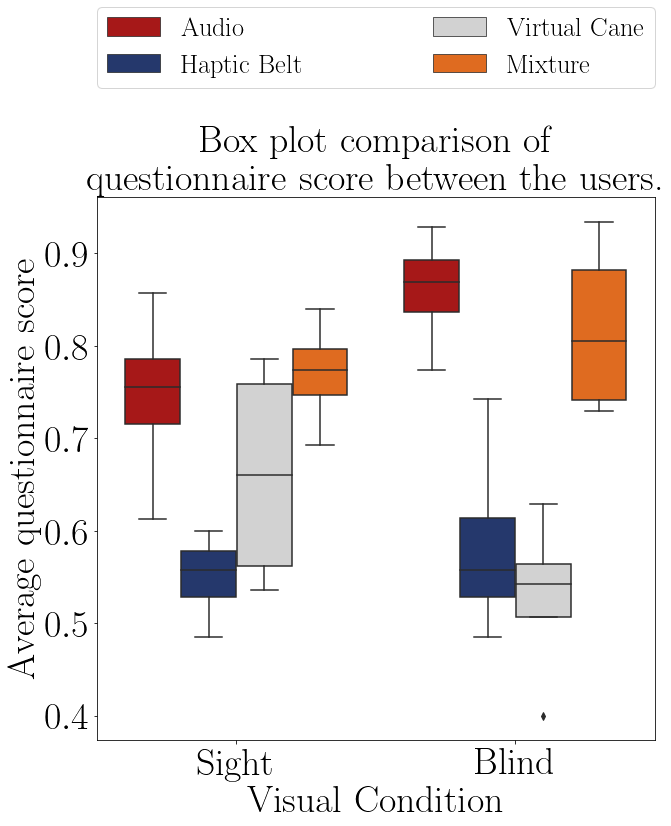
\includegraphics[width = 0.5\linewidth]{Resultados/Questionario/Figuras/png/boxplot_questionnaire_scene.png}
    %\resizebox{0.5\linewidth}{!}{
    %%% Creator: Matplotlib, PGF backend
%%
%% To include the figure in your LaTeX document, write
%%   \input{<filename>.pgf}
%%
%% Make sure the required packages are loaded in your preamble
%%   \usepackage{pgf}
%%
%% and, on pdftex
%%   \usepackage[utf8]{inputenc}\DeclareUnicodeCharacter{2212}{-}
%%
%% or, on luatex and xetex
%%   \usepackage{unicode-math}
%%
%% Figures using additional raster images can only be included by \input if
%% they are in the same directory as the main LaTeX file. For loading figures
%% from other directories you can use the `import` package
%%   \usepackage{import}
%%
%% and then include the figures with
%%   \import{<path to file>}{<filename>.pgf}
%%
%% Matplotlib used the following preamble
%%   \usepackage{url}
%%   \usepackage{unicode-math}
%%   \setmainfont{DejaVu Serif}
%%   \usepackage{fontspec}
%%
\begingroup%
\makeatletter%
\begin{pgfpicture}%
\pgfpathrectangle{\pgfpointorigin}{\pgfqpoint{12.196638in}{14.528848in}}%
\pgfusepath{use as bounding box, clip}%
\begin{pgfscope}%
\pgfsetbuttcap%
\pgfsetmiterjoin%
\pgfsetlinewidth{0.000000pt}%
\definecolor{currentstroke}{rgb}{1.000000,1.000000,1.000000}%
\pgfsetstrokecolor{currentstroke}%
\pgfsetstrokeopacity{0.000000}%
\pgfsetdash{}{0pt}%
\pgfpathmoveto{\pgfqpoint{0.000000in}{0.000000in}}%
\pgfpathlineto{\pgfqpoint{12.196638in}{0.000000in}}%
\pgfpathlineto{\pgfqpoint{12.196638in}{14.528848in}}%
\pgfpathlineto{\pgfqpoint{0.000000in}{14.528848in}}%
\pgfpathclose%
\pgfusepath{}%
\end{pgfscope}%
\begin{pgfscope}%
\pgfsetbuttcap%
\pgfsetmiterjoin%
\definecolor{currentfill}{rgb}{1.000000,1.000000,1.000000}%
\pgfsetfillcolor{currentfill}%
\pgfsetlinewidth{0.000000pt}%
\definecolor{currentstroke}{rgb}{0.000000,0.000000,0.000000}%
\pgfsetstrokecolor{currentstroke}%
\pgfsetstrokeopacity{0.000000}%
\pgfsetdash{}{0pt}%
\pgfpathmoveto{\pgfqpoint{1.246638in}{1.110648in}}%
\pgfpathlineto{\pgfqpoint{12.096638in}{1.110648in}}%
\pgfpathlineto{\pgfqpoint{12.096638in}{11.680648in}}%
\pgfpathlineto{\pgfqpoint{1.246638in}{11.680648in}}%
\pgfpathclose%
\pgfusepath{fill}%
\end{pgfscope}%
\begin{pgfscope}%
\pgfpathrectangle{\pgfqpoint{1.246638in}{1.110648in}}{\pgfqpoint{10.850000in}{10.570000in}}%
\pgfusepath{clip}%
\pgfsetbuttcap%
\pgfsetmiterjoin%
\definecolor{currentfill}{rgb}{0.651961,0.093137,0.093137}%
\pgfsetfillcolor{currentfill}%
\pgfsetlinewidth{1.505625pt}%
\definecolor{currentstroke}{rgb}{0.168627,0.168627,0.168627}%
\pgfsetstrokecolor{currentstroke}%
\pgfsetdash{}{0pt}%
\pgfpathmoveto{\pgfqpoint{1.799988in}{4.877546in}}%
\pgfpathlineto{\pgfqpoint{2.863288in}{4.877546in}}%
\pgfpathlineto{\pgfqpoint{2.863288in}{8.797921in}}%
\pgfpathlineto{\pgfqpoint{1.799988in}{8.797921in}}%
\pgfpathlineto{\pgfqpoint{1.799988in}{4.877546in}}%
\pgfpathclose%
\pgfusepath{stroke,fill}%
\end{pgfscope}%
\begin{pgfscope}%
\pgfpathrectangle{\pgfqpoint{1.246638in}{1.110648in}}{\pgfqpoint{10.850000in}{10.570000in}}%
\pgfusepath{clip}%
\pgfsetbuttcap%
\pgfsetmiterjoin%
\definecolor{currentfill}{rgb}{0.144608,0.218137,0.424020}%
\pgfsetfillcolor{currentfill}%
\pgfsetlinewidth{1.505625pt}%
\definecolor{currentstroke}{rgb}{0.168627,0.168627,0.168627}%
\pgfsetstrokecolor{currentstroke}%
\pgfsetdash{}{0pt}%
\pgfpathmoveto{\pgfqpoint{2.884988in}{6.929487in}}%
\pgfpathlineto{\pgfqpoint{3.948288in}{6.929487in}}%
\pgfpathlineto{\pgfqpoint{3.948288in}{8.130623in}}%
\pgfpathlineto{\pgfqpoint{2.884988in}{8.130623in}}%
\pgfpathlineto{\pgfqpoint{2.884988in}{6.929487in}}%
\pgfpathclose%
\pgfusepath{stroke,fill}%
\end{pgfscope}%
\begin{pgfscope}%
\pgfpathrectangle{\pgfqpoint{1.246638in}{1.110648in}}{\pgfqpoint{10.850000in}{10.570000in}}%
\pgfusepath{clip}%
\pgfsetbuttcap%
\pgfsetmiterjoin%
\definecolor{currentfill}{rgb}{0.823529,0.823529,0.823529}%
\pgfsetfillcolor{currentfill}%
\pgfsetlinewidth{1.505625pt}%
\definecolor{currentstroke}{rgb}{0.168627,0.168627,0.168627}%
\pgfsetstrokecolor{currentstroke}%
\pgfsetdash{}{0pt}%
\pgfpathmoveto{\pgfqpoint{3.969988in}{3.960011in}}%
\pgfpathlineto{\pgfqpoint{5.033288in}{3.960011in}}%
\pgfpathlineto{\pgfqpoint{5.033288in}{5.294607in}}%
\pgfpathlineto{\pgfqpoint{3.969988in}{5.294607in}}%
\pgfpathlineto{\pgfqpoint{3.969988in}{3.960011in}}%
\pgfpathclose%
\pgfusepath{stroke,fill}%
\end{pgfscope}%
\begin{pgfscope}%
\pgfpathrectangle{\pgfqpoint{1.246638in}{1.110648in}}{\pgfqpoint{10.850000in}{10.570000in}}%
\pgfusepath{clip}%
\pgfsetbuttcap%
\pgfsetmiterjoin%
\definecolor{currentfill}{rgb}{0.875000,0.419118,0.125000}%
\pgfsetfillcolor{currentfill}%
\pgfsetlinewidth{1.505625pt}%
\definecolor{currentstroke}{rgb}{0.168627,0.168627,0.168627}%
\pgfsetstrokecolor{currentstroke}%
\pgfsetdash{}{0pt}%
\pgfpathmoveto{\pgfqpoint{5.054988in}{5.667509in}}%
\pgfpathlineto{\pgfqpoint{6.118288in}{5.667509in}}%
\pgfpathlineto{\pgfqpoint{6.118288in}{8.407846in}}%
\pgfpathlineto{\pgfqpoint{5.054988in}{8.407846in}}%
\pgfpathlineto{\pgfqpoint{5.054988in}{5.667509in}}%
\pgfpathclose%
\pgfusepath{stroke,fill}%
\end{pgfscope}%
\begin{pgfscope}%
\pgfpathrectangle{\pgfqpoint{1.246638in}{1.110648in}}{\pgfqpoint{10.850000in}{10.570000in}}%
\pgfusepath{clip}%
\pgfsetbuttcap%
\pgfsetmiterjoin%
\definecolor{currentfill}{rgb}{0.651961,0.093137,0.093137}%
\pgfsetfillcolor{currentfill}%
\pgfsetlinewidth{1.505625pt}%
\definecolor{currentstroke}{rgb}{0.168627,0.168627,0.168627}%
\pgfsetstrokecolor{currentstroke}%
\pgfsetdash{}{0pt}%
\pgfpathmoveto{\pgfqpoint{7.224988in}{5.739472in}}%
\pgfpathlineto{\pgfqpoint{8.288288in}{5.739472in}}%
\pgfpathlineto{\pgfqpoint{8.288288in}{7.796974in}}%
\pgfpathlineto{\pgfqpoint{7.224988in}{7.796974in}}%
\pgfpathlineto{\pgfqpoint{7.224988in}{5.739472in}}%
\pgfpathclose%
\pgfusepath{stroke,fill}%
\end{pgfscope}%
\begin{pgfscope}%
\pgfpathrectangle{\pgfqpoint{1.246638in}{1.110648in}}{\pgfqpoint{10.850000in}{10.570000in}}%
\pgfusepath{clip}%
\pgfsetbuttcap%
\pgfsetmiterjoin%
\definecolor{currentfill}{rgb}{0.144608,0.218137,0.424020}%
\pgfsetfillcolor{currentfill}%
\pgfsetlinewidth{1.505625pt}%
\definecolor{currentstroke}{rgb}{0.168627,0.168627,0.168627}%
\pgfsetstrokecolor{currentstroke}%
\pgfsetdash{}{0pt}%
\pgfpathmoveto{\pgfqpoint{8.309988in}{7.196406in}}%
\pgfpathlineto{\pgfqpoint{9.373288in}{7.196406in}}%
\pgfpathlineto{\pgfqpoint{9.373288in}{8.797921in}}%
\pgfpathlineto{\pgfqpoint{8.309988in}{8.797921in}}%
\pgfpathlineto{\pgfqpoint{8.309988in}{7.196406in}}%
\pgfpathclose%
\pgfusepath{stroke,fill}%
\end{pgfscope}%
\begin{pgfscope}%
\pgfpathrectangle{\pgfqpoint{1.246638in}{1.110648in}}{\pgfqpoint{10.850000in}{10.570000in}}%
\pgfusepath{clip}%
\pgfsetbuttcap%
\pgfsetmiterjoin%
\definecolor{currentfill}{rgb}{0.823529,0.823529,0.823529}%
\pgfsetfillcolor{currentfill}%
\pgfsetlinewidth{1.505625pt}%
\definecolor{currentstroke}{rgb}{0.168627,0.168627,0.168627}%
\pgfsetstrokecolor{currentstroke}%
\pgfsetdash{}{0pt}%
\pgfpathmoveto{\pgfqpoint{9.394988in}{2.391861in}}%
\pgfpathlineto{\pgfqpoint{10.458288in}{2.391861in}}%
\pgfpathlineto{\pgfqpoint{10.458288in}{3.459537in}}%
\pgfpathlineto{\pgfqpoint{9.394988in}{3.459537in}}%
\pgfpathlineto{\pgfqpoint{9.394988in}{2.391861in}}%
\pgfpathclose%
\pgfusepath{stroke,fill}%
\end{pgfscope}%
\begin{pgfscope}%
\pgfpathrectangle{\pgfqpoint{1.246638in}{1.110648in}}{\pgfqpoint{10.850000in}{10.570000in}}%
\pgfusepath{clip}%
\pgfsetbuttcap%
\pgfsetmiterjoin%
\definecolor{currentfill}{rgb}{0.875000,0.419118,0.125000}%
\pgfsetfillcolor{currentfill}%
\pgfsetlinewidth{1.505625pt}%
\definecolor{currentstroke}{rgb}{0.168627,0.168627,0.168627}%
\pgfsetstrokecolor{currentstroke}%
\pgfsetdash{}{0pt}%
\pgfpathmoveto{\pgfqpoint{10.479988in}{7.064800in}}%
\pgfpathlineto{\pgfqpoint{11.543288in}{7.064800in}}%
\pgfpathlineto{\pgfqpoint{11.543288in}{8.758668in}}%
\pgfpathlineto{\pgfqpoint{10.479988in}{8.758668in}}%
\pgfpathlineto{\pgfqpoint{10.479988in}{7.064800in}}%
\pgfpathclose%
\pgfusepath{stroke,fill}%
\end{pgfscope}%
\begin{pgfscope}%
\pgfpathrectangle{\pgfqpoint{1.246638in}{1.110648in}}{\pgfqpoint{10.850000in}{10.570000in}}%
\pgfusepath{clip}%
\pgfsetbuttcap%
\pgfsetmiterjoin%
\definecolor{currentfill}{rgb}{0.651961,0.093137,0.093137}%
\pgfsetfillcolor{currentfill}%
\pgfsetlinewidth{0.752812pt}%
\definecolor{currentstroke}{rgb}{0.168627,0.168627,0.168627}%
\pgfsetstrokecolor{currentstroke}%
\pgfsetdash{}{0pt}%
\pgfpathmoveto{\pgfqpoint{3.959138in}{-5.882634in}}%
\pgfpathlineto{\pgfqpoint{3.959138in}{-5.882634in}}%
\pgfpathlineto{\pgfqpoint{3.959138in}{-5.882634in}}%
\pgfpathlineto{\pgfqpoint{3.959138in}{-5.882634in}}%
\pgfpathclose%
\pgfusepath{stroke,fill}%
\end{pgfscope}%
\begin{pgfscope}%
\pgfpathrectangle{\pgfqpoint{1.246638in}{1.110648in}}{\pgfqpoint{10.850000in}{10.570000in}}%
\pgfusepath{clip}%
\pgfsetbuttcap%
\pgfsetmiterjoin%
\definecolor{currentfill}{rgb}{0.144608,0.218137,0.424020}%
\pgfsetfillcolor{currentfill}%
\pgfsetlinewidth{0.752812pt}%
\definecolor{currentstroke}{rgb}{0.168627,0.168627,0.168627}%
\pgfsetstrokecolor{currentstroke}%
\pgfsetdash{}{0pt}%
\pgfpathmoveto{\pgfqpoint{3.959138in}{-5.882634in}}%
\pgfpathlineto{\pgfqpoint{3.959138in}{-5.882634in}}%
\pgfpathlineto{\pgfqpoint{3.959138in}{-5.882634in}}%
\pgfpathlineto{\pgfqpoint{3.959138in}{-5.882634in}}%
\pgfpathclose%
\pgfusepath{stroke,fill}%
\end{pgfscope}%
\begin{pgfscope}%
\pgfpathrectangle{\pgfqpoint{1.246638in}{1.110648in}}{\pgfqpoint{10.850000in}{10.570000in}}%
\pgfusepath{clip}%
\pgfsetbuttcap%
\pgfsetmiterjoin%
\definecolor{currentfill}{rgb}{0.823529,0.823529,0.823529}%
\pgfsetfillcolor{currentfill}%
\pgfsetlinewidth{0.752812pt}%
\definecolor{currentstroke}{rgb}{0.168627,0.168627,0.168627}%
\pgfsetstrokecolor{currentstroke}%
\pgfsetdash{}{0pt}%
\pgfpathmoveto{\pgfqpoint{3.959138in}{-5.882634in}}%
\pgfpathlineto{\pgfqpoint{3.959138in}{-5.882634in}}%
\pgfpathlineto{\pgfqpoint{3.959138in}{-5.882634in}}%
\pgfpathlineto{\pgfqpoint{3.959138in}{-5.882634in}}%
\pgfpathclose%
\pgfusepath{stroke,fill}%
\end{pgfscope}%
\begin{pgfscope}%
\pgfpathrectangle{\pgfqpoint{1.246638in}{1.110648in}}{\pgfqpoint{10.850000in}{10.570000in}}%
\pgfusepath{clip}%
\pgfsetbuttcap%
\pgfsetmiterjoin%
\definecolor{currentfill}{rgb}{0.875000,0.419118,0.125000}%
\pgfsetfillcolor{currentfill}%
\pgfsetlinewidth{0.752812pt}%
\definecolor{currentstroke}{rgb}{0.168627,0.168627,0.168627}%
\pgfsetstrokecolor{currentstroke}%
\pgfsetdash{}{0pt}%
\pgfpathmoveto{\pgfqpoint{3.959138in}{-5.882634in}}%
\pgfpathlineto{\pgfqpoint{3.959138in}{-5.882634in}}%
\pgfpathlineto{\pgfqpoint{3.959138in}{-5.882634in}}%
\pgfpathlineto{\pgfqpoint{3.959138in}{-5.882634in}}%
\pgfpathclose%
\pgfusepath{stroke,fill}%
\end{pgfscope}%
\begin{pgfscope}%
\pgfsetbuttcap%
\pgfsetroundjoin%
\definecolor{currentfill}{rgb}{0.000000,0.000000,0.000000}%
\pgfsetfillcolor{currentfill}%
\pgfsetlinewidth{0.803000pt}%
\definecolor{currentstroke}{rgb}{0.000000,0.000000,0.000000}%
\pgfsetstrokecolor{currentstroke}%
\pgfsetdash{}{0pt}%
\pgfsys@defobject{currentmarker}{\pgfqpoint{0.000000in}{-0.048611in}}{\pgfqpoint{0.000000in}{0.000000in}}{%
\pgfpathmoveto{\pgfqpoint{0.000000in}{0.000000in}}%
\pgfpathlineto{\pgfqpoint{0.000000in}{-0.048611in}}%
\pgfusepath{stroke,fill}%
}%
\begin{pgfscope}%
\pgfsys@transformshift{3.959138in}{1.110648in}%
\pgfsys@useobject{currentmarker}{}%
\end{pgfscope}%
\end{pgfscope}%
\begin{pgfscope}%
\definecolor{textcolor}{rgb}{0.000000,0.000000,0.000000}%
\pgfsetstrokecolor{textcolor}%
\pgfsetfillcolor{textcolor}%
\pgftext[x=3.959138in,y=1.013426in,,top]{\color{textcolor}\rmfamily\fontsize{31.680000}{38.016000}\selectfont Sight}%
\end{pgfscope}%
\begin{pgfscope}%
\pgfsetbuttcap%
\pgfsetroundjoin%
\definecolor{currentfill}{rgb}{0.000000,0.000000,0.000000}%
\pgfsetfillcolor{currentfill}%
\pgfsetlinewidth{0.803000pt}%
\definecolor{currentstroke}{rgb}{0.000000,0.000000,0.000000}%
\pgfsetstrokecolor{currentstroke}%
\pgfsetdash{}{0pt}%
\pgfsys@defobject{currentmarker}{\pgfqpoint{0.000000in}{-0.048611in}}{\pgfqpoint{0.000000in}{0.000000in}}{%
\pgfpathmoveto{\pgfqpoint{0.000000in}{0.000000in}}%
\pgfpathlineto{\pgfqpoint{0.000000in}{-0.048611in}}%
\pgfusepath{stroke,fill}%
}%
\begin{pgfscope}%
\pgfsys@transformshift{9.384138in}{1.110648in}%
\pgfsys@useobject{currentmarker}{}%
\end{pgfscope}%
\end{pgfscope}%
\begin{pgfscope}%
\definecolor{textcolor}{rgb}{0.000000,0.000000,0.000000}%
\pgfsetstrokecolor{textcolor}%
\pgfsetfillcolor{textcolor}%
\pgftext[x=9.384138in,y=1.013426in,,top]{\color{textcolor}\rmfamily\fontsize{31.680000}{38.016000}\selectfont Blind}%
\end{pgfscope}%
\begin{pgfscope}%
\definecolor{textcolor}{rgb}{0.000000,0.000000,0.000000}%
\pgfsetstrokecolor{textcolor}%
\pgfsetfillcolor{textcolor}%
\pgftext[x=6.671638in,y=0.525820in,,top]{\color{textcolor}\rmfamily\fontsize{31.680000}{38.016000}\selectfont Visual Condition}%
\end{pgfscope}%
\begin{pgfscope}%
\pgfsetbuttcap%
\pgfsetroundjoin%
\definecolor{currentfill}{rgb}{0.000000,0.000000,0.000000}%
\pgfsetfillcolor{currentfill}%
\pgfsetlinewidth{0.803000pt}%
\definecolor{currentstroke}{rgb}{0.000000,0.000000,0.000000}%
\pgfsetstrokecolor{currentstroke}%
\pgfsetdash{}{0pt}%
\pgfsys@defobject{currentmarker}{\pgfqpoint{-0.048611in}{0.000000in}}{\pgfqpoint{-0.000000in}{0.000000in}}{%
\pgfpathmoveto{\pgfqpoint{-0.000000in}{0.000000in}}%
\pgfpathlineto{\pgfqpoint{-0.048611in}{0.000000in}}%
\pgfusepath{stroke,fill}%
}%
\begin{pgfscope}%
\pgfsys@transformshift{1.246638in}{1.591103in}%
\pgfsys@useobject{currentmarker}{}%
\end{pgfscope}%
\end{pgfscope}%
\begin{pgfscope}%
\definecolor{textcolor}{rgb}{0.000000,0.000000,0.000000}%
\pgfsetstrokecolor{textcolor}%
\pgfsetfillcolor{textcolor}%
\pgftext[x=0.587096in, y=1.423955in, left, base]{\color{textcolor}\rmfamily\fontsize{31.680000}{38.016000}\selectfont \(\displaystyle {0.4}\)}%
\end{pgfscope}%
\begin{pgfscope}%
\pgfsetbuttcap%
\pgfsetroundjoin%
\definecolor{currentfill}{rgb}{0.000000,0.000000,0.000000}%
\pgfsetfillcolor{currentfill}%
\pgfsetlinewidth{0.803000pt}%
\definecolor{currentstroke}{rgb}{0.000000,0.000000,0.000000}%
\pgfsetstrokecolor{currentstroke}%
\pgfsetdash{}{0pt}%
\pgfsys@defobject{currentmarker}{\pgfqpoint{-0.048611in}{0.000000in}}{\pgfqpoint{-0.000000in}{0.000000in}}{%
\pgfpathmoveto{\pgfqpoint{-0.000000in}{0.000000in}}%
\pgfpathlineto{\pgfqpoint{-0.048611in}{0.000000in}}%
\pgfusepath{stroke,fill}%
}%
\begin{pgfscope}%
\pgfsys@transformshift{1.246638in}{3.459537in}%
\pgfsys@useobject{currentmarker}{}%
\end{pgfscope}%
\end{pgfscope}%
\begin{pgfscope}%
\definecolor{textcolor}{rgb}{0.000000,0.000000,0.000000}%
\pgfsetstrokecolor{textcolor}%
\pgfsetfillcolor{textcolor}%
\pgftext[x=0.587096in, y=3.292389in, left, base]{\color{textcolor}\rmfamily\fontsize{31.680000}{38.016000}\selectfont \(\displaystyle {0.5}\)}%
\end{pgfscope}%
\begin{pgfscope}%
\pgfsetbuttcap%
\pgfsetroundjoin%
\definecolor{currentfill}{rgb}{0.000000,0.000000,0.000000}%
\pgfsetfillcolor{currentfill}%
\pgfsetlinewidth{0.803000pt}%
\definecolor{currentstroke}{rgb}{0.000000,0.000000,0.000000}%
\pgfsetstrokecolor{currentstroke}%
\pgfsetdash{}{0pt}%
\pgfsys@defobject{currentmarker}{\pgfqpoint{-0.048611in}{0.000000in}}{\pgfqpoint{-0.000000in}{0.000000in}}{%
\pgfpathmoveto{\pgfqpoint{-0.000000in}{0.000000in}}%
\pgfpathlineto{\pgfqpoint{-0.048611in}{0.000000in}}%
\pgfusepath{stroke,fill}%
}%
\begin{pgfscope}%
\pgfsys@transformshift{1.246638in}{5.327972in}%
\pgfsys@useobject{currentmarker}{}%
\end{pgfscope}%
\end{pgfscope}%
\begin{pgfscope}%
\definecolor{textcolor}{rgb}{0.000000,0.000000,0.000000}%
\pgfsetstrokecolor{textcolor}%
\pgfsetfillcolor{textcolor}%
\pgftext[x=0.587096in, y=5.160823in, left, base]{\color{textcolor}\rmfamily\fontsize{31.680000}{38.016000}\selectfont \(\displaystyle {0.6}\)}%
\end{pgfscope}%
\begin{pgfscope}%
\pgfsetbuttcap%
\pgfsetroundjoin%
\definecolor{currentfill}{rgb}{0.000000,0.000000,0.000000}%
\pgfsetfillcolor{currentfill}%
\pgfsetlinewidth{0.803000pt}%
\definecolor{currentstroke}{rgb}{0.000000,0.000000,0.000000}%
\pgfsetstrokecolor{currentstroke}%
\pgfsetdash{}{0pt}%
\pgfsys@defobject{currentmarker}{\pgfqpoint{-0.048611in}{0.000000in}}{\pgfqpoint{-0.000000in}{0.000000in}}{%
\pgfpathmoveto{\pgfqpoint{-0.000000in}{0.000000in}}%
\pgfpathlineto{\pgfqpoint{-0.048611in}{0.000000in}}%
\pgfusepath{stroke,fill}%
}%
\begin{pgfscope}%
\pgfsys@transformshift{1.246638in}{7.196406in}%
\pgfsys@useobject{currentmarker}{}%
\end{pgfscope}%
\end{pgfscope}%
\begin{pgfscope}%
\definecolor{textcolor}{rgb}{0.000000,0.000000,0.000000}%
\pgfsetstrokecolor{textcolor}%
\pgfsetfillcolor{textcolor}%
\pgftext[x=0.581376in, y=7.029258in, left, base]{\color{textcolor}\rmfamily\fontsize{31.680000}{38.016000}\selectfont \(\displaystyle {0.7}\)}%
\end{pgfscope}%
\begin{pgfscope}%
\pgfsetbuttcap%
\pgfsetroundjoin%
\definecolor{currentfill}{rgb}{0.000000,0.000000,0.000000}%
\pgfsetfillcolor{currentfill}%
\pgfsetlinewidth{0.803000pt}%
\definecolor{currentstroke}{rgb}{0.000000,0.000000,0.000000}%
\pgfsetstrokecolor{currentstroke}%
\pgfsetdash{}{0pt}%
\pgfsys@defobject{currentmarker}{\pgfqpoint{-0.048611in}{0.000000in}}{\pgfqpoint{-0.000000in}{0.000000in}}{%
\pgfpathmoveto{\pgfqpoint{-0.000000in}{0.000000in}}%
\pgfpathlineto{\pgfqpoint{-0.048611in}{0.000000in}}%
\pgfusepath{stroke,fill}%
}%
\begin{pgfscope}%
\pgfsys@transformshift{1.246638in}{9.064840in}%
\pgfsys@useobject{currentmarker}{}%
\end{pgfscope}%
\end{pgfscope}%
\begin{pgfscope}%
\definecolor{textcolor}{rgb}{0.000000,0.000000,0.000000}%
\pgfsetstrokecolor{textcolor}%
\pgfsetfillcolor{textcolor}%
\pgftext[x=0.587096in, y=8.897692in, left, base]{\color{textcolor}\rmfamily\fontsize{31.680000}{38.016000}\selectfont \(\displaystyle {0.8}\)}%
\end{pgfscope}%
\begin{pgfscope}%
\pgfsetbuttcap%
\pgfsetroundjoin%
\definecolor{currentfill}{rgb}{0.000000,0.000000,0.000000}%
\pgfsetfillcolor{currentfill}%
\pgfsetlinewidth{0.803000pt}%
\definecolor{currentstroke}{rgb}{0.000000,0.000000,0.000000}%
\pgfsetstrokecolor{currentstroke}%
\pgfsetdash{}{0pt}%
\pgfsys@defobject{currentmarker}{\pgfqpoint{-0.048611in}{0.000000in}}{\pgfqpoint{-0.000000in}{0.000000in}}{%
\pgfpathmoveto{\pgfqpoint{-0.000000in}{0.000000in}}%
\pgfpathlineto{\pgfqpoint{-0.048611in}{0.000000in}}%
\pgfusepath{stroke,fill}%
}%
\begin{pgfscope}%
\pgfsys@transformshift{1.246638in}{10.933275in}%
\pgfsys@useobject{currentmarker}{}%
\end{pgfscope}%
\end{pgfscope}%
\begin{pgfscope}%
\definecolor{textcolor}{rgb}{0.000000,0.000000,0.000000}%
\pgfsetstrokecolor{textcolor}%
\pgfsetfillcolor{textcolor}%
\pgftext[x=0.587096in, y=10.766126in, left, base]{\color{textcolor}\rmfamily\fontsize{31.680000}{38.016000}\selectfont \(\displaystyle {0.9}\)}%
\end{pgfscope}%
\begin{pgfscope}%
\definecolor{textcolor}{rgb}{0.000000,0.000000,0.000000}%
\pgfsetstrokecolor{textcolor}%
\pgfsetfillcolor{textcolor}%
\pgftext[x=0.525820in,y=6.395648in,,bottom,rotate=90.000000]{\color{textcolor}\rmfamily\fontsize{31.680000}{38.016000}\selectfont Average questionnaire score}%
\end{pgfscope}%
\begin{pgfscope}%
\pgfpathrectangle{\pgfqpoint{1.246638in}{1.110648in}}{\pgfqpoint{10.850000in}{10.570000in}}%
\pgfusepath{clip}%
\pgfsetrectcap%
\pgfsetroundjoin%
\pgfsetlinewidth{1.505625pt}%
\definecolor{currentstroke}{rgb}{0.168627,0.168627,0.168627}%
\pgfsetstrokecolor{currentstroke}%
\pgfsetdash{}{0pt}%
\pgfpathmoveto{\pgfqpoint{2.331638in}{4.877546in}}%
\pgfpathlineto{\pgfqpoint{2.331638in}{2.792239in}}%
\pgfusepath{stroke}%
\end{pgfscope}%
\begin{pgfscope}%
\pgfpathrectangle{\pgfqpoint{1.246638in}{1.110648in}}{\pgfqpoint{10.850000in}{10.570000in}}%
\pgfusepath{clip}%
\pgfsetrectcap%
\pgfsetroundjoin%
\pgfsetlinewidth{1.505625pt}%
\definecolor{currentstroke}{rgb}{0.168627,0.168627,0.168627}%
\pgfsetstrokecolor{currentstroke}%
\pgfsetdash{}{0pt}%
\pgfpathmoveto{\pgfqpoint{2.331638in}{8.797921in}}%
\pgfpathlineto{\pgfqpoint{2.331638in}{10.132517in}}%
\pgfusepath{stroke}%
\end{pgfscope}%
\begin{pgfscope}%
\pgfpathrectangle{\pgfqpoint{1.246638in}{1.110648in}}{\pgfqpoint{10.850000in}{10.570000in}}%
\pgfusepath{clip}%
\pgfsetrectcap%
\pgfsetroundjoin%
\pgfsetlinewidth{1.505625pt}%
\definecolor{currentstroke}{rgb}{0.168627,0.168627,0.168627}%
\pgfsetstrokecolor{currentstroke}%
\pgfsetdash{}{0pt}%
\pgfpathmoveto{\pgfqpoint{2.065813in}{2.792239in}}%
\pgfpathlineto{\pgfqpoint{2.597463in}{2.792239in}}%
\pgfusepath{stroke}%
\end{pgfscope}%
\begin{pgfscope}%
\pgfpathrectangle{\pgfqpoint{1.246638in}{1.110648in}}{\pgfqpoint{10.850000in}{10.570000in}}%
\pgfusepath{clip}%
\pgfsetrectcap%
\pgfsetroundjoin%
\pgfsetlinewidth{1.505625pt}%
\definecolor{currentstroke}{rgb}{0.168627,0.168627,0.168627}%
\pgfsetstrokecolor{currentstroke}%
\pgfsetdash{}{0pt}%
\pgfpathmoveto{\pgfqpoint{2.065813in}{10.132517in}}%
\pgfpathlineto{\pgfqpoint{2.597463in}{10.132517in}}%
\pgfusepath{stroke}%
\end{pgfscope}%
\begin{pgfscope}%
\pgfpathrectangle{\pgfqpoint{1.246638in}{1.110648in}}{\pgfqpoint{10.850000in}{10.570000in}}%
\pgfusepath{clip}%
\pgfsetrectcap%
\pgfsetroundjoin%
\pgfsetlinewidth{1.505625pt}%
\definecolor{currentstroke}{rgb}{0.168627,0.168627,0.168627}%
\pgfsetstrokecolor{currentstroke}%
\pgfsetdash{}{0pt}%
\pgfpathmoveto{\pgfqpoint{3.416638in}{6.929487in}}%
\pgfpathlineto{\pgfqpoint{3.416638in}{5.327972in}}%
\pgfusepath{stroke}%
\end{pgfscope}%
\begin{pgfscope}%
\pgfpathrectangle{\pgfqpoint{1.246638in}{1.110648in}}{\pgfqpoint{10.850000in}{10.570000in}}%
\pgfusepath{clip}%
\pgfsetrectcap%
\pgfsetroundjoin%
\pgfsetlinewidth{1.505625pt}%
\definecolor{currentstroke}{rgb}{0.168627,0.168627,0.168627}%
\pgfsetstrokecolor{currentstroke}%
\pgfsetdash{}{0pt}%
\pgfpathmoveto{\pgfqpoint{3.416638in}{8.130623in}}%
\pgfpathlineto{\pgfqpoint{3.416638in}{8.531002in}}%
\pgfusepath{stroke}%
\end{pgfscope}%
\begin{pgfscope}%
\pgfpathrectangle{\pgfqpoint{1.246638in}{1.110648in}}{\pgfqpoint{10.850000in}{10.570000in}}%
\pgfusepath{clip}%
\pgfsetrectcap%
\pgfsetroundjoin%
\pgfsetlinewidth{1.505625pt}%
\definecolor{currentstroke}{rgb}{0.168627,0.168627,0.168627}%
\pgfsetstrokecolor{currentstroke}%
\pgfsetdash{}{0pt}%
\pgfpathmoveto{\pgfqpoint{3.150813in}{5.327972in}}%
\pgfpathlineto{\pgfqpoint{3.682463in}{5.327972in}}%
\pgfusepath{stroke}%
\end{pgfscope}%
\begin{pgfscope}%
\pgfpathrectangle{\pgfqpoint{1.246638in}{1.110648in}}{\pgfqpoint{10.850000in}{10.570000in}}%
\pgfusepath{clip}%
\pgfsetrectcap%
\pgfsetroundjoin%
\pgfsetlinewidth{1.505625pt}%
\definecolor{currentstroke}{rgb}{0.168627,0.168627,0.168627}%
\pgfsetstrokecolor{currentstroke}%
\pgfsetdash{}{0pt}%
\pgfpathmoveto{\pgfqpoint{3.150813in}{8.531002in}}%
\pgfpathlineto{\pgfqpoint{3.682463in}{8.531002in}}%
\pgfusepath{stroke}%
\end{pgfscope}%
\begin{pgfscope}%
\pgfpathrectangle{\pgfqpoint{1.246638in}{1.110648in}}{\pgfqpoint{10.850000in}{10.570000in}}%
\pgfusepath{clip}%
\pgfsetrectcap%
\pgfsetroundjoin%
\pgfsetlinewidth{1.505625pt}%
\definecolor{currentstroke}{rgb}{0.168627,0.168627,0.168627}%
\pgfsetstrokecolor{currentstroke}%
\pgfsetdash{}{0pt}%
\pgfpathmoveto{\pgfqpoint{4.501638in}{3.960011in}}%
\pgfpathlineto{\pgfqpoint{4.501638in}{3.459537in}}%
\pgfusepath{stroke}%
\end{pgfscope}%
\begin{pgfscope}%
\pgfpathrectangle{\pgfqpoint{1.246638in}{1.110648in}}{\pgfqpoint{10.850000in}{10.570000in}}%
\pgfusepath{clip}%
\pgfsetrectcap%
\pgfsetroundjoin%
\pgfsetlinewidth{1.505625pt}%
\definecolor{currentstroke}{rgb}{0.168627,0.168627,0.168627}%
\pgfsetstrokecolor{currentstroke}%
\pgfsetdash{}{0pt}%
\pgfpathmoveto{\pgfqpoint{4.501638in}{5.294607in}}%
\pgfpathlineto{\pgfqpoint{4.501638in}{6.796027in}}%
\pgfusepath{stroke}%
\end{pgfscope}%
\begin{pgfscope}%
\pgfpathrectangle{\pgfqpoint{1.246638in}{1.110648in}}{\pgfqpoint{10.850000in}{10.570000in}}%
\pgfusepath{clip}%
\pgfsetrectcap%
\pgfsetroundjoin%
\pgfsetlinewidth{1.505625pt}%
\definecolor{currentstroke}{rgb}{0.168627,0.168627,0.168627}%
\pgfsetstrokecolor{currentstroke}%
\pgfsetdash{}{0pt}%
\pgfpathmoveto{\pgfqpoint{4.235813in}{3.459537in}}%
\pgfpathlineto{\pgfqpoint{4.767463in}{3.459537in}}%
\pgfusepath{stroke}%
\end{pgfscope}%
\begin{pgfscope}%
\pgfpathrectangle{\pgfqpoint{1.246638in}{1.110648in}}{\pgfqpoint{10.850000in}{10.570000in}}%
\pgfusepath{clip}%
\pgfsetrectcap%
\pgfsetroundjoin%
\pgfsetlinewidth{1.505625pt}%
\definecolor{currentstroke}{rgb}{0.168627,0.168627,0.168627}%
\pgfsetstrokecolor{currentstroke}%
\pgfsetdash{}{0pt}%
\pgfpathmoveto{\pgfqpoint{4.235813in}{6.796027in}}%
\pgfpathlineto{\pgfqpoint{4.767463in}{6.796027in}}%
\pgfusepath{stroke}%
\end{pgfscope}%
\begin{pgfscope}%
\pgfpathrectangle{\pgfqpoint{1.246638in}{1.110648in}}{\pgfqpoint{10.850000in}{10.570000in}}%
\pgfusepath{clip}%
\pgfsetrectcap%
\pgfsetroundjoin%
\pgfsetlinewidth{1.505625pt}%
\definecolor{currentstroke}{rgb}{0.168627,0.168627,0.168627}%
\pgfsetstrokecolor{currentstroke}%
\pgfsetdash{}{0pt}%
\pgfpathmoveto{\pgfqpoint{5.586638in}{5.667509in}}%
\pgfpathlineto{\pgfqpoint{5.586638in}{4.519364in}}%
\pgfusepath{stroke}%
\end{pgfscope}%
\begin{pgfscope}%
\pgfpathrectangle{\pgfqpoint{1.246638in}{1.110648in}}{\pgfqpoint{10.850000in}{10.570000in}}%
\pgfusepath{clip}%
\pgfsetrectcap%
\pgfsetroundjoin%
\pgfsetlinewidth{1.505625pt}%
\definecolor{currentstroke}{rgb}{0.168627,0.168627,0.168627}%
\pgfsetstrokecolor{currentstroke}%
\pgfsetdash{}{0pt}%
\pgfpathmoveto{\pgfqpoint{5.586638in}{8.407846in}}%
\pgfpathlineto{\pgfqpoint{5.586638in}{10.299342in}}%
\pgfusepath{stroke}%
\end{pgfscope}%
\begin{pgfscope}%
\pgfpathrectangle{\pgfqpoint{1.246638in}{1.110648in}}{\pgfqpoint{10.850000in}{10.570000in}}%
\pgfusepath{clip}%
\pgfsetrectcap%
\pgfsetroundjoin%
\pgfsetlinewidth{1.505625pt}%
\definecolor{currentstroke}{rgb}{0.168627,0.168627,0.168627}%
\pgfsetstrokecolor{currentstroke}%
\pgfsetdash{}{0pt}%
\pgfpathmoveto{\pgfqpoint{5.320813in}{4.519364in}}%
\pgfpathlineto{\pgfqpoint{5.852463in}{4.519364in}}%
\pgfusepath{stroke}%
\end{pgfscope}%
\begin{pgfscope}%
\pgfpathrectangle{\pgfqpoint{1.246638in}{1.110648in}}{\pgfqpoint{10.850000in}{10.570000in}}%
\pgfusepath{clip}%
\pgfsetrectcap%
\pgfsetroundjoin%
\pgfsetlinewidth{1.505625pt}%
\definecolor{currentstroke}{rgb}{0.168627,0.168627,0.168627}%
\pgfsetstrokecolor{currentstroke}%
\pgfsetdash{}{0pt}%
\pgfpathmoveto{\pgfqpoint{5.320813in}{10.299342in}}%
\pgfpathlineto{\pgfqpoint{5.852463in}{10.299342in}}%
\pgfusepath{stroke}%
\end{pgfscope}%
\begin{pgfscope}%
\pgfpathrectangle{\pgfqpoint{1.246638in}{1.110648in}}{\pgfqpoint{10.850000in}{10.570000in}}%
\pgfusepath{clip}%
\pgfsetrectcap%
\pgfsetroundjoin%
\pgfsetlinewidth{1.505625pt}%
\definecolor{currentstroke}{rgb}{0.168627,0.168627,0.168627}%
\pgfsetstrokecolor{currentstroke}%
\pgfsetdash{}{0pt}%
\pgfpathmoveto{\pgfqpoint{7.756638in}{5.739472in}}%
\pgfpathlineto{\pgfqpoint{7.756638in}{5.238999in}}%
\pgfusepath{stroke}%
\end{pgfscope}%
\begin{pgfscope}%
\pgfpathrectangle{\pgfqpoint{1.246638in}{1.110648in}}{\pgfqpoint{10.850000in}{10.570000in}}%
\pgfusepath{clip}%
\pgfsetrectcap%
\pgfsetroundjoin%
\pgfsetlinewidth{1.505625pt}%
\definecolor{currentstroke}{rgb}{0.168627,0.168627,0.168627}%
\pgfsetstrokecolor{currentstroke}%
\pgfsetdash{}{0pt}%
\pgfpathmoveto{\pgfqpoint{7.756638in}{7.796974in}}%
\pgfpathlineto{\pgfqpoint{7.756638in}{10.132517in}}%
\pgfusepath{stroke}%
\end{pgfscope}%
\begin{pgfscope}%
\pgfpathrectangle{\pgfqpoint{1.246638in}{1.110648in}}{\pgfqpoint{10.850000in}{10.570000in}}%
\pgfusepath{clip}%
\pgfsetrectcap%
\pgfsetroundjoin%
\pgfsetlinewidth{1.505625pt}%
\definecolor{currentstroke}{rgb}{0.168627,0.168627,0.168627}%
\pgfsetstrokecolor{currentstroke}%
\pgfsetdash{}{0pt}%
\pgfpathmoveto{\pgfqpoint{7.490813in}{5.238999in}}%
\pgfpathlineto{\pgfqpoint{8.022463in}{5.238999in}}%
\pgfusepath{stroke}%
\end{pgfscope}%
\begin{pgfscope}%
\pgfpathrectangle{\pgfqpoint{1.246638in}{1.110648in}}{\pgfqpoint{10.850000in}{10.570000in}}%
\pgfusepath{clip}%
\pgfsetrectcap%
\pgfsetroundjoin%
\pgfsetlinewidth{1.505625pt}%
\definecolor{currentstroke}{rgb}{0.168627,0.168627,0.168627}%
\pgfsetstrokecolor{currentstroke}%
\pgfsetdash{}{0pt}%
\pgfpathmoveto{\pgfqpoint{7.490813in}{10.132517in}}%
\pgfpathlineto{\pgfqpoint{8.022463in}{10.132517in}}%
\pgfusepath{stroke}%
\end{pgfscope}%
\begin{pgfscope}%
\pgfpathrectangle{\pgfqpoint{1.246638in}{1.110648in}}{\pgfqpoint{10.850000in}{10.570000in}}%
\pgfusepath{clip}%
\pgfsetrectcap%
\pgfsetroundjoin%
\pgfsetlinewidth{1.505625pt}%
\definecolor{currentstroke}{rgb}{0.168627,0.168627,0.168627}%
\pgfsetstrokecolor{currentstroke}%
\pgfsetdash{}{0pt}%
\pgfpathmoveto{\pgfqpoint{8.841638in}{7.196406in}}%
\pgfpathlineto{\pgfqpoint{8.841638in}{6.395648in}}%
\pgfusepath{stroke}%
\end{pgfscope}%
\begin{pgfscope}%
\pgfpathrectangle{\pgfqpoint{1.246638in}{1.110648in}}{\pgfqpoint{10.850000in}{10.570000in}}%
\pgfusepath{clip}%
\pgfsetrectcap%
\pgfsetroundjoin%
\pgfsetlinewidth{1.505625pt}%
\definecolor{currentstroke}{rgb}{0.168627,0.168627,0.168627}%
\pgfsetstrokecolor{currentstroke}%
\pgfsetdash{}{0pt}%
\pgfpathmoveto{\pgfqpoint{8.841638in}{8.797921in}}%
\pgfpathlineto{\pgfqpoint{8.841638in}{8.797921in}}%
\pgfusepath{stroke}%
\end{pgfscope}%
\begin{pgfscope}%
\pgfpathrectangle{\pgfqpoint{1.246638in}{1.110648in}}{\pgfqpoint{10.850000in}{10.570000in}}%
\pgfusepath{clip}%
\pgfsetrectcap%
\pgfsetroundjoin%
\pgfsetlinewidth{1.505625pt}%
\definecolor{currentstroke}{rgb}{0.168627,0.168627,0.168627}%
\pgfsetstrokecolor{currentstroke}%
\pgfsetdash{}{0pt}%
\pgfpathmoveto{\pgfqpoint{8.575813in}{6.395648in}}%
\pgfpathlineto{\pgfqpoint{9.107463in}{6.395648in}}%
\pgfusepath{stroke}%
\end{pgfscope}%
\begin{pgfscope}%
\pgfpathrectangle{\pgfqpoint{1.246638in}{1.110648in}}{\pgfqpoint{10.850000in}{10.570000in}}%
\pgfusepath{clip}%
\pgfsetrectcap%
\pgfsetroundjoin%
\pgfsetlinewidth{1.505625pt}%
\definecolor{currentstroke}{rgb}{0.168627,0.168627,0.168627}%
\pgfsetstrokecolor{currentstroke}%
\pgfsetdash{}{0pt}%
\pgfpathmoveto{\pgfqpoint{8.575813in}{8.797921in}}%
\pgfpathlineto{\pgfqpoint{9.107463in}{8.797921in}}%
\pgfusepath{stroke}%
\end{pgfscope}%
\begin{pgfscope}%
\pgfpathrectangle{\pgfqpoint{1.246638in}{1.110648in}}{\pgfqpoint{10.850000in}{10.570000in}}%
\pgfusepath{clip}%
\pgfsetbuttcap%
\pgfsetmiterjoin%
\definecolor{currentfill}{rgb}{0.168627,0.168627,0.168627}%
\pgfsetfillcolor{currentfill}%
\pgfsetlinewidth{1.003750pt}%
\definecolor{currentstroke}{rgb}{0.168627,0.168627,0.168627}%
\pgfsetstrokecolor{currentstroke}%
\pgfsetdash{}{0pt}%
\pgfsys@defobject{currentmarker}{\pgfqpoint{-0.029463in}{-0.049105in}}{\pgfqpoint{0.029463in}{0.049105in}}{%
\pgfpathmoveto{\pgfqpoint{0.000000in}{-0.049105in}}%
\pgfpathlineto{\pgfqpoint{0.029463in}{0.000000in}}%
\pgfpathlineto{\pgfqpoint{0.000000in}{0.049105in}}%
\pgfpathlineto{\pgfqpoint{-0.029463in}{0.000000in}}%
\pgfpathclose%
\pgfusepath{stroke,fill}%
}%
\begin{pgfscope}%
\pgfsys@transformshift{8.841638in}{11.200194in}%
\pgfsys@useobject{currentmarker}{}%
\end{pgfscope}%
\end{pgfscope}%
\begin{pgfscope}%
\pgfpathrectangle{\pgfqpoint{1.246638in}{1.110648in}}{\pgfqpoint{10.850000in}{10.570000in}}%
\pgfusepath{clip}%
\pgfsetrectcap%
\pgfsetroundjoin%
\pgfsetlinewidth{1.505625pt}%
\definecolor{currentstroke}{rgb}{0.168627,0.168627,0.168627}%
\pgfsetstrokecolor{currentstroke}%
\pgfsetdash{}{0pt}%
\pgfpathmoveto{\pgfqpoint{9.926638in}{2.391861in}}%
\pgfpathlineto{\pgfqpoint{9.926638in}{1.591103in}}%
\pgfusepath{stroke}%
\end{pgfscope}%
\begin{pgfscope}%
\pgfpathrectangle{\pgfqpoint{1.246638in}{1.110648in}}{\pgfqpoint{10.850000in}{10.570000in}}%
\pgfusepath{clip}%
\pgfsetrectcap%
\pgfsetroundjoin%
\pgfsetlinewidth{1.505625pt}%
\definecolor{currentstroke}{rgb}{0.168627,0.168627,0.168627}%
\pgfsetstrokecolor{currentstroke}%
\pgfsetdash{}{0pt}%
\pgfpathmoveto{\pgfqpoint{9.926638in}{3.459537in}}%
\pgfpathlineto{\pgfqpoint{9.926638in}{4.260295in}}%
\pgfusepath{stroke}%
\end{pgfscope}%
\begin{pgfscope}%
\pgfpathrectangle{\pgfqpoint{1.246638in}{1.110648in}}{\pgfqpoint{10.850000in}{10.570000in}}%
\pgfusepath{clip}%
\pgfsetrectcap%
\pgfsetroundjoin%
\pgfsetlinewidth{1.505625pt}%
\definecolor{currentstroke}{rgb}{0.168627,0.168627,0.168627}%
\pgfsetstrokecolor{currentstroke}%
\pgfsetdash{}{0pt}%
\pgfpathmoveto{\pgfqpoint{9.660813in}{1.591103in}}%
\pgfpathlineto{\pgfqpoint{10.192463in}{1.591103in}}%
\pgfusepath{stroke}%
\end{pgfscope}%
\begin{pgfscope}%
\pgfpathrectangle{\pgfqpoint{1.246638in}{1.110648in}}{\pgfqpoint{10.850000in}{10.570000in}}%
\pgfusepath{clip}%
\pgfsetrectcap%
\pgfsetroundjoin%
\pgfsetlinewidth{1.505625pt}%
\definecolor{currentstroke}{rgb}{0.168627,0.168627,0.168627}%
\pgfsetstrokecolor{currentstroke}%
\pgfsetdash{}{0pt}%
\pgfpathmoveto{\pgfqpoint{9.660813in}{4.260295in}}%
\pgfpathlineto{\pgfqpoint{10.192463in}{4.260295in}}%
\pgfusepath{stroke}%
\end{pgfscope}%
\begin{pgfscope}%
\pgfpathrectangle{\pgfqpoint{1.246638in}{1.110648in}}{\pgfqpoint{10.850000in}{10.570000in}}%
\pgfusepath{clip}%
\pgfsetrectcap%
\pgfsetroundjoin%
\pgfsetlinewidth{1.505625pt}%
\definecolor{currentstroke}{rgb}{0.168627,0.168627,0.168627}%
\pgfsetstrokecolor{currentstroke}%
\pgfsetdash{}{0pt}%
\pgfpathmoveto{\pgfqpoint{11.011638in}{7.064800in}}%
\pgfpathlineto{\pgfqpoint{11.011638in}{5.535576in}}%
\pgfusepath{stroke}%
\end{pgfscope}%
\begin{pgfscope}%
\pgfpathrectangle{\pgfqpoint{1.246638in}{1.110648in}}{\pgfqpoint{10.850000in}{10.570000in}}%
\pgfusepath{clip}%
\pgfsetrectcap%
\pgfsetroundjoin%
\pgfsetlinewidth{1.505625pt}%
\definecolor{currentstroke}{rgb}{0.168627,0.168627,0.168627}%
\pgfsetstrokecolor{currentstroke}%
\pgfsetdash{}{0pt}%
\pgfpathmoveto{\pgfqpoint{11.011638in}{8.758668in}}%
\pgfpathlineto{\pgfqpoint{11.011638in}{9.975506in}}%
\pgfusepath{stroke}%
\end{pgfscope}%
\begin{pgfscope}%
\pgfpathrectangle{\pgfqpoint{1.246638in}{1.110648in}}{\pgfqpoint{10.850000in}{10.570000in}}%
\pgfusepath{clip}%
\pgfsetrectcap%
\pgfsetroundjoin%
\pgfsetlinewidth{1.505625pt}%
\definecolor{currentstroke}{rgb}{0.168627,0.168627,0.168627}%
\pgfsetstrokecolor{currentstroke}%
\pgfsetdash{}{0pt}%
\pgfpathmoveto{\pgfqpoint{10.745813in}{5.535576in}}%
\pgfpathlineto{\pgfqpoint{11.277463in}{5.535576in}}%
\pgfusepath{stroke}%
\end{pgfscope}%
\begin{pgfscope}%
\pgfpathrectangle{\pgfqpoint{1.246638in}{1.110648in}}{\pgfqpoint{10.850000in}{10.570000in}}%
\pgfusepath{clip}%
\pgfsetrectcap%
\pgfsetroundjoin%
\pgfsetlinewidth{1.505625pt}%
\definecolor{currentstroke}{rgb}{0.168627,0.168627,0.168627}%
\pgfsetstrokecolor{currentstroke}%
\pgfsetdash{}{0pt}%
\pgfpathmoveto{\pgfqpoint{10.745813in}{9.975506in}}%
\pgfpathlineto{\pgfqpoint{11.277463in}{9.975506in}}%
\pgfusepath{stroke}%
\end{pgfscope}%
\begin{pgfscope}%
\pgfpathrectangle{\pgfqpoint{1.246638in}{1.110648in}}{\pgfqpoint{10.850000in}{10.570000in}}%
\pgfusepath{clip}%
\pgfsetrectcap%
\pgfsetroundjoin%
\pgfsetlinewidth{1.505625pt}%
\definecolor{currentstroke}{rgb}{0.168627,0.168627,0.168627}%
\pgfsetstrokecolor{currentstroke}%
\pgfsetdash{}{0pt}%
\pgfpathmoveto{\pgfqpoint{1.799988in}{6.962852in}}%
\pgfpathlineto{\pgfqpoint{2.863288in}{6.962852in}}%
\pgfusepath{stroke}%
\end{pgfscope}%
\begin{pgfscope}%
\pgfpathrectangle{\pgfqpoint{1.246638in}{1.110648in}}{\pgfqpoint{10.850000in}{10.570000in}}%
\pgfusepath{clip}%
\pgfsetrectcap%
\pgfsetroundjoin%
\pgfsetlinewidth{1.505625pt}%
\definecolor{currentstroke}{rgb}{0.168627,0.168627,0.168627}%
\pgfsetstrokecolor{currentstroke}%
\pgfsetdash{}{0pt}%
\pgfpathmoveto{\pgfqpoint{2.884988in}{7.730244in}}%
\pgfpathlineto{\pgfqpoint{3.948288in}{7.730244in}}%
\pgfusepath{stroke}%
\end{pgfscope}%
\begin{pgfscope}%
\pgfpathrectangle{\pgfqpoint{1.246638in}{1.110648in}}{\pgfqpoint{10.850000in}{10.570000in}}%
\pgfusepath{clip}%
\pgfsetrectcap%
\pgfsetroundjoin%
\pgfsetlinewidth{1.505625pt}%
\definecolor{currentstroke}{rgb}{0.168627,0.168627,0.168627}%
\pgfsetstrokecolor{currentstroke}%
\pgfsetdash{}{0pt}%
\pgfpathmoveto{\pgfqpoint{3.969988in}{4.460484in}}%
\pgfpathlineto{\pgfqpoint{5.033288in}{4.460484in}}%
\pgfusepath{stroke}%
\end{pgfscope}%
\begin{pgfscope}%
\pgfpathrectangle{\pgfqpoint{1.246638in}{1.110648in}}{\pgfqpoint{10.850000in}{10.570000in}}%
\pgfusepath{clip}%
\pgfsetrectcap%
\pgfsetroundjoin%
\pgfsetlinewidth{1.505625pt}%
\definecolor{currentstroke}{rgb}{0.168627,0.168627,0.168627}%
\pgfsetstrokecolor{currentstroke}%
\pgfsetdash{}{0pt}%
\pgfpathmoveto{\pgfqpoint{5.054988in}{6.913786in}}%
\pgfpathlineto{\pgfqpoint{6.118288in}{6.913786in}}%
\pgfusepath{stroke}%
\end{pgfscope}%
\begin{pgfscope}%
\pgfpathrectangle{\pgfqpoint{1.246638in}{1.110648in}}{\pgfqpoint{10.850000in}{10.570000in}}%
\pgfusepath{clip}%
\pgfsetrectcap%
\pgfsetroundjoin%
\pgfsetlinewidth{1.505625pt}%
\definecolor{currentstroke}{rgb}{0.168627,0.168627,0.168627}%
\pgfsetstrokecolor{currentstroke}%
\pgfsetdash{}{0pt}%
\pgfpathmoveto{\pgfqpoint{7.224988in}{6.462378in}}%
\pgfpathlineto{\pgfqpoint{8.288288in}{6.462378in}}%
\pgfusepath{stroke}%
\end{pgfscope}%
\begin{pgfscope}%
\pgfpathrectangle{\pgfqpoint{1.246638in}{1.110648in}}{\pgfqpoint{10.850000in}{10.570000in}}%
\pgfusepath{clip}%
\pgfsetrectcap%
\pgfsetroundjoin%
\pgfsetlinewidth{1.505625pt}%
\definecolor{currentstroke}{rgb}{0.168627,0.168627,0.168627}%
\pgfsetstrokecolor{currentstroke}%
\pgfsetdash{}{0pt}%
\pgfpathmoveto{\pgfqpoint{8.309988in}{7.730244in}}%
\pgfpathlineto{\pgfqpoint{9.373288in}{7.730244in}}%
\pgfusepath{stroke}%
\end{pgfscope}%
\begin{pgfscope}%
\pgfpathrectangle{\pgfqpoint{1.246638in}{1.110648in}}{\pgfqpoint{10.850000in}{10.570000in}}%
\pgfusepath{clip}%
\pgfsetrectcap%
\pgfsetroundjoin%
\pgfsetlinewidth{1.505625pt}%
\definecolor{currentstroke}{rgb}{0.168627,0.168627,0.168627}%
\pgfsetstrokecolor{currentstroke}%
\pgfsetdash{}{0pt}%
\pgfpathmoveto{\pgfqpoint{9.394988in}{2.925699in}}%
\pgfpathlineto{\pgfqpoint{10.458288in}{2.925699in}}%
\pgfusepath{stroke}%
\end{pgfscope}%
\begin{pgfscope}%
\pgfpathrectangle{\pgfqpoint{1.246638in}{1.110648in}}{\pgfqpoint{10.850000in}{10.570000in}}%
\pgfusepath{clip}%
\pgfsetrectcap%
\pgfsetroundjoin%
\pgfsetlinewidth{1.505625pt}%
\definecolor{currentstroke}{rgb}{0.168627,0.168627,0.168627}%
\pgfsetstrokecolor{currentstroke}%
\pgfsetdash{}{0pt}%
\pgfpathmoveto{\pgfqpoint{10.479988in}{7.963799in}}%
\pgfpathlineto{\pgfqpoint{11.543288in}{7.963799in}}%
\pgfusepath{stroke}%
\end{pgfscope}%
\begin{pgfscope}%
\pgfsetrectcap%
\pgfsetmiterjoin%
\pgfsetlinewidth{0.803000pt}%
\definecolor{currentstroke}{rgb}{0.000000,0.000000,0.000000}%
\pgfsetstrokecolor{currentstroke}%
\pgfsetdash{}{0pt}%
\pgfpathmoveto{\pgfqpoint{1.246638in}{1.110648in}}%
\pgfpathlineto{\pgfqpoint{1.246638in}{11.680648in}}%
\pgfusepath{stroke}%
\end{pgfscope}%
\begin{pgfscope}%
\pgfsetrectcap%
\pgfsetmiterjoin%
\pgfsetlinewidth{0.803000pt}%
\definecolor{currentstroke}{rgb}{0.000000,0.000000,0.000000}%
\pgfsetstrokecolor{currentstroke}%
\pgfsetdash{}{0pt}%
\pgfpathmoveto{\pgfqpoint{12.096638in}{1.110648in}}%
\pgfpathlineto{\pgfqpoint{12.096638in}{11.680648in}}%
\pgfusepath{stroke}%
\end{pgfscope}%
\begin{pgfscope}%
\pgfsetrectcap%
\pgfsetmiterjoin%
\pgfsetlinewidth{0.803000pt}%
\definecolor{currentstroke}{rgb}{0.000000,0.000000,0.000000}%
\pgfsetstrokecolor{currentstroke}%
\pgfsetdash{}{0pt}%
\pgfpathmoveto{\pgfqpoint{1.246638in}{1.110648in}}%
\pgfpathlineto{\pgfqpoint{12.096638in}{1.110648in}}%
\pgfusepath{stroke}%
\end{pgfscope}%
\begin{pgfscope}%
\pgfsetrectcap%
\pgfsetmiterjoin%
\pgfsetlinewidth{0.803000pt}%
\definecolor{currentstroke}{rgb}{0.000000,0.000000,0.000000}%
\pgfsetstrokecolor{currentstroke}%
\pgfsetdash{}{0pt}%
\pgfpathmoveto{\pgfqpoint{1.246638in}{11.680648in}}%
\pgfpathlineto{\pgfqpoint{12.096638in}{11.680648in}}%
\pgfusepath{stroke}%
\end{pgfscope}%
\begin{pgfscope}%
\definecolor{textcolor}{rgb}{0.000000,0.000000,0.000000}%
\pgfsetstrokecolor{textcolor}%
\pgfsetfillcolor{textcolor}%
\pgftext[x=3.500415in, y=12.381692in, left, base]{\color{textcolor}\rmfamily\fontsize{38.016000}{45.619200}\selectfont Box plot comparison of }%
\end{pgfscope}%
\begin{pgfscope}%
\definecolor{textcolor}{rgb}{0.000000,0.000000,0.000000}%
\pgfsetstrokecolor{textcolor}%
\pgfsetfillcolor{textcolor}%
\pgftext[x=1.387254in, y=11.790476in, left, base]{\color{textcolor}\rmfamily\fontsize{38.016000}{45.619200}\selectfont questionnaire score between the users.}%
\end{pgfscope}%
\begin{pgfscope}%
\pgfsetbuttcap%
\pgfsetmiterjoin%
\definecolor{currentfill}{rgb}{1.000000,1.000000,1.000000}%
\pgfsetfillcolor{currentfill}%
\pgfsetfillopacity{0.800000}%
\pgfsetlinewidth{1.003750pt}%
\definecolor{currentstroke}{rgb}{0.800000,0.800000,0.800000}%
\pgfsetstrokecolor{currentstroke}%
\pgfsetstrokeopacity{0.800000}%
\pgfsetdash{}{0pt}%
\pgfpathmoveto{\pgfqpoint{9.108489in}{12.543237in}}%
\pgfpathlineto{\pgfqpoint{12.035527in}{12.543237in}}%
\pgfpathquadraticcurveto{\pgfqpoint{12.096638in}{12.543237in}}{\pgfqpoint{12.096638in}{12.604348in}}%
\pgfpathlineto{\pgfqpoint{12.096638in}{14.367737in}}%
\pgfpathquadraticcurveto{\pgfqpoint{12.096638in}{14.428848in}}{\pgfqpoint{12.035527in}{14.428848in}}%
\pgfpathlineto{\pgfqpoint{9.108489in}{14.428848in}}%
\pgfpathquadraticcurveto{\pgfqpoint{9.047378in}{14.428848in}}{\pgfqpoint{9.047378in}{14.367737in}}%
\pgfpathlineto{\pgfqpoint{9.047378in}{12.604348in}}%
\pgfpathquadraticcurveto{\pgfqpoint{9.047378in}{12.543237in}}{\pgfqpoint{9.108489in}{12.543237in}}%
\pgfpathclose%
\pgfusepath{stroke,fill}%
\end{pgfscope}%
\begin{pgfscope}%
\pgfsetbuttcap%
\pgfsetmiterjoin%
\definecolor{currentfill}{rgb}{0.651961,0.093137,0.093137}%
\pgfsetfillcolor{currentfill}%
\pgfsetlinewidth{0.752812pt}%
\definecolor{currentstroke}{rgb}{0.168627,0.168627,0.168627}%
\pgfsetstrokecolor{currentstroke}%
\pgfsetdash{}{0pt}%
\pgfpathmoveto{\pgfqpoint{9.169600in}{14.074476in}}%
\pgfpathlineto{\pgfqpoint{9.780712in}{14.074476in}}%
\pgfpathlineto{\pgfqpoint{9.780712in}{14.288365in}}%
\pgfpathlineto{\pgfqpoint{9.169600in}{14.288365in}}%
\pgfpathclose%
\pgfusepath{stroke,fill}%
\end{pgfscope}%
\begin{pgfscope}%
\definecolor{textcolor}{rgb}{0.000000,0.000000,0.000000}%
\pgfsetstrokecolor{textcolor}%
\pgfsetfillcolor{textcolor}%
\pgftext[x=10.025156in,y=14.074476in,left,base]{\color{textcolor}\rmfamily\fontsize{22.000000}{26.400000}\selectfont Audio}%
\end{pgfscope}%
\begin{pgfscope}%
\pgfsetbuttcap%
\pgfsetmiterjoin%
\definecolor{currentfill}{rgb}{0.144608,0.218137,0.424020}%
\pgfsetfillcolor{currentfill}%
\pgfsetlinewidth{0.752812pt}%
\definecolor{currentstroke}{rgb}{0.168627,0.168627,0.168627}%
\pgfsetstrokecolor{currentstroke}%
\pgfsetdash{}{0pt}%
\pgfpathmoveto{\pgfqpoint{9.169600in}{13.625990in}}%
\pgfpathlineto{\pgfqpoint{9.780712in}{13.625990in}}%
\pgfpathlineto{\pgfqpoint{9.780712in}{13.839878in}}%
\pgfpathlineto{\pgfqpoint{9.169600in}{13.839878in}}%
\pgfpathclose%
\pgfusepath{stroke,fill}%
\end{pgfscope}%
\begin{pgfscope}%
\definecolor{textcolor}{rgb}{0.000000,0.000000,0.000000}%
\pgfsetstrokecolor{textcolor}%
\pgfsetfillcolor{textcolor}%
\pgftext[x=10.025156in,y=13.625990in,left,base]{\color{textcolor}\rmfamily\fontsize{22.000000}{26.400000}\selectfont Haptic Belt}%
\end{pgfscope}%
\begin{pgfscope}%
\pgfsetbuttcap%
\pgfsetmiterjoin%
\definecolor{currentfill}{rgb}{0.823529,0.823529,0.823529}%
\pgfsetfillcolor{currentfill}%
\pgfsetlinewidth{0.752812pt}%
\definecolor{currentstroke}{rgb}{0.168627,0.168627,0.168627}%
\pgfsetstrokecolor{currentstroke}%
\pgfsetdash{}{0pt}%
\pgfpathmoveto{\pgfqpoint{9.169600in}{13.177503in}}%
\pgfpathlineto{\pgfqpoint{9.780712in}{13.177503in}}%
\pgfpathlineto{\pgfqpoint{9.780712in}{13.391392in}}%
\pgfpathlineto{\pgfqpoint{9.169600in}{13.391392in}}%
\pgfpathclose%
\pgfusepath{stroke,fill}%
\end{pgfscope}%
\begin{pgfscope}%
\definecolor{textcolor}{rgb}{0.000000,0.000000,0.000000}%
\pgfsetstrokecolor{textcolor}%
\pgfsetfillcolor{textcolor}%
\pgftext[x=10.025156in,y=13.177503in,left,base]{\color{textcolor}\rmfamily\fontsize{22.000000}{26.400000}\selectfont Virtual Cane}%
\end{pgfscope}%
\begin{pgfscope}%
\pgfsetbuttcap%
\pgfsetmiterjoin%
\definecolor{currentfill}{rgb}{0.875000,0.419118,0.125000}%
\pgfsetfillcolor{currentfill}%
\pgfsetlinewidth{0.752812pt}%
\definecolor{currentstroke}{rgb}{0.168627,0.168627,0.168627}%
\pgfsetstrokecolor{currentstroke}%
\pgfsetdash{}{0pt}%
\pgfpathmoveto{\pgfqpoint{9.169600in}{12.729017in}}%
\pgfpathlineto{\pgfqpoint{9.780712in}{12.729017in}}%
\pgfpathlineto{\pgfqpoint{9.780712in}{12.942906in}}%
\pgfpathlineto{\pgfqpoint{9.169600in}{12.942906in}}%
\pgfpathclose%
\pgfusepath{stroke,fill}%
\end{pgfscope}%
\begin{pgfscope}%
\definecolor{textcolor}{rgb}{0.000000,0.000000,0.000000}%
\pgfsetstrokecolor{textcolor}%
\pgfsetfillcolor{textcolor}%
\pgftext[x=10.025156in,y=12.729017in,left,base]{\color{textcolor}\rmfamily\fontsize{22.000000}{26.400000}\selectfont Mixture}%
\end{pgfscope}%
\end{pgfpicture}%
\makeatother%
\endgroup%

    %}
    \caption{Boxplot of the average questionnaire score of each group.}
    \label{fig:boxplot_questionnaire_scene}
\end{figure}

The Shapiro–Wilk normality test on the Table \ref{tab:shapiro_questionnaires} shows that these data are normally distributed, with a p-value higher than 0.05, then it is possible to perform the following test to check if there is a significant difference between the methods


\begin{table}[!htb]
\centering
\caption{Shapiro test p-value for the questionnaires score for each method and visual condition.}
\label{tab:shapiro_questionnaires}
\begin{tabular}{lr}
\toprule
            Method &  Shapiro P-Value \\
\midrule
       Audio blind &            0.400 \\
       Audio sight &            0.882 \\
 Haptic Belt blind &            0.414 \\
 Haptic Belt sight &            0.369 \\
Virtual Cane blind &            0.995 \\
Virtual Cane sight &            0.577 \\
     Mixture blind &            0.966 \\
     Mixture sight &            0.925 \\
\bottomrule
\end{tabular}
\end{table}



The Table \ref{tab:anova_questionnaire} shows the Anova test p-value of the Sagat score average of the "blind" sample between the guidance methods presented in the Table \ref{tab:questionnaire_average}. The p-value indicates that all scores are significantly different from each other. That means that the highest scores shown in Table \ref{tab:questionnaire_average_group}, which are the "Haptic Belt" and the "Mixture" methods were the most favorite by the participant.


\begin{table}[!htb]
\centering
\caption{Anova p-value for the questionnaire score on each method for blinded users.}
\label{tab:anova_questionnaire}
\begin{tabular}{lrrrrr}
\toprule
         Source &  Squared sum &  DOF & Squared average &     F & \begin{tabular}[c]{@{}l@{}}P-Value \\ $(F_{0} > F)$\end{tabular} \\
\midrule
Between factors &        0.207 &    3 &           0.069 & 7.080 &                                                            0.005 \\
 Inside factors &        0.117 &   12 &           0.010 &       &                                                                  \\
          Total &        0.324 &   15 &                 &       &                                                                  \\
\bottomrule
\end{tabular}
\end{table}



\FloatBarrier